\documentclass[]{book}
\usepackage{lmodern}
\usepackage{amssymb,amsmath}
\usepackage{ifxetex,ifluatex}
\usepackage{fixltx2e} % provides \textsubscript
\ifnum 0\ifxetex 1\fi\ifluatex 1\fi=0 % if pdftex
  \usepackage[T1]{fontenc}
  \usepackage[utf8]{inputenc}
\else % if luatex or xelatex
  \ifxetex
    \usepackage{mathspec}
  \else
    \usepackage{fontspec}
  \fi
  \defaultfontfeatures{Ligatures=TeX,Scale=MatchLowercase}
\fi
% use upquote if available, for straight quotes in verbatim environments
\IfFileExists{upquote.sty}{\usepackage{upquote}}{}
% use microtype if available
\IfFileExists{microtype.sty}{%
\usepackage{microtype}
\UseMicrotypeSet[protrusion]{basicmath} % disable protrusion for tt fonts
}{}
\usepackage{hyperref}
\hypersetup{unicode=true,
            pdftitle={Visualization, transformation and reporting with the tidyverse},
            pdfauthor={Kirill Müller, Tobias Schieferdecker, Patrick Schratz},
            pdfborder={0 0 0},
            breaklinks=true}
\urlstyle{same}  % don't use monospace font for urls
\usepackage{natbib}
\bibliographystyle{apa-old.cls}
\usepackage{color}
\usepackage{fancyvrb}
\newcommand{\VerbBar}{|}
\newcommand{\VERB}{\Verb[commandchars=\\\{\}]}
\DefineVerbatimEnvironment{Highlighting}{Verbatim}{commandchars=\\\{\}}
% Add ',fontsize=\small' for more characters per line
\newenvironment{Shaded}{}{}
\newcommand{\AlertTok}[1]{\textcolor[rgb]{1.00,0.00,0.00}{#1}}
\newcommand{\AnnotationTok}[1]{\textcolor[rgb]{0.00,0.50,0.00}{#1}}
\newcommand{\AttributeTok}[1]{#1}
\newcommand{\BaseNTok}[1]{#1}
\newcommand{\BuiltInTok}[1]{#1}
\newcommand{\CharTok}[1]{\textcolor[rgb]{0.00,0.50,0.50}{#1}}
\newcommand{\CommentTok}[1]{\textcolor[rgb]{0.00,0.50,0.00}{#1}}
\newcommand{\CommentVarTok}[1]{\textcolor[rgb]{0.00,0.50,0.00}{#1}}
\newcommand{\ConstantTok}[1]{#1}
\newcommand{\ControlFlowTok}[1]{\textcolor[rgb]{0.00,0.00,1.00}{#1}}
\newcommand{\DataTypeTok}[1]{#1}
\newcommand{\DecValTok}[1]{#1}
\newcommand{\DocumentationTok}[1]{\textcolor[rgb]{0.00,0.50,0.00}{#1}}
\newcommand{\ErrorTok}[1]{\textcolor[rgb]{1.00,0.00,0.00}{\textbf{#1}}}
\newcommand{\ExtensionTok}[1]{#1}
\newcommand{\FloatTok}[1]{#1}
\newcommand{\FunctionTok}[1]{#1}
\newcommand{\ImportTok}[1]{#1}
\newcommand{\InformationTok}[1]{\textcolor[rgb]{0.00,0.50,0.00}{#1}}
\newcommand{\KeywordTok}[1]{\textcolor[rgb]{0.00,0.00,1.00}{#1}}
\newcommand{\NormalTok}[1]{#1}
\newcommand{\OperatorTok}[1]{#1}
\newcommand{\OtherTok}[1]{\textcolor[rgb]{1.00,0.25,0.00}{#1}}
\newcommand{\PreprocessorTok}[1]{\textcolor[rgb]{1.00,0.25,0.00}{#1}}
\newcommand{\RegionMarkerTok}[1]{#1}
\newcommand{\SpecialCharTok}[1]{\textcolor[rgb]{0.00,0.50,0.50}{#1}}
\newcommand{\SpecialStringTok}[1]{\textcolor[rgb]{0.00,0.50,0.50}{#1}}
\newcommand{\StringTok}[1]{\textcolor[rgb]{0.00,0.50,0.50}{#1}}
\newcommand{\VariableTok}[1]{#1}
\newcommand{\VerbatimStringTok}[1]{\textcolor[rgb]{0.00,0.50,0.50}{#1}}
\newcommand{\WarningTok}[1]{\textcolor[rgb]{0.00,0.50,0.00}{\textbf{#1}}}
\usepackage{longtable,booktabs}
\usepackage{graphicx}
% grffile has become a legacy package: https://ctan.org/pkg/grffile
\IfFileExists{grffile.sty}{%
\usepackage{grffile}
}{}
\makeatletter
\def\maxwidth{\ifdim\Gin@nat@width>\linewidth\linewidth\else\Gin@nat@width\fi}
\def\maxheight{\ifdim\Gin@nat@height>\textheight\textheight\else\Gin@nat@height\fi}
\makeatother
% Scale images if necessary, so that they will not overflow the page
% margins by default, and it is still possible to overwrite the defaults
% using explicit options in \includegraphics[width, height, ...]{}
\setkeys{Gin}{width=\maxwidth,height=\maxheight,keepaspectratio}
\IfFileExists{parskip.sty}{%
\usepackage{parskip}
}{% else
\setlength{\parindent}{0pt}
\setlength{\parskip}{6pt plus 2pt minus 1pt}
}
\setlength{\emergencystretch}{3em}  % prevent overfull lines
\providecommand{\tightlist}{%
  \setlength{\itemsep}{0pt}\setlength{\parskip}{0pt}}
\setcounter{secnumdepth}{5}
% Redefines (sub)paragraphs to behave more like sections
\ifx\paragraph\undefined\else
\let\oldparagraph\paragraph
\renewcommand{\paragraph}[1]{\oldparagraph{#1}\mbox{}}
\fi
\ifx\subparagraph\undefined\else
\let\oldsubparagraph\subparagraph
\renewcommand{\subparagraph}[1]{\oldsubparagraph{#1}\mbox{}}
\fi

%%% Use protect on footnotes to avoid problems with footnotes in titles
\let\rmarkdownfootnote\footnote%
\def\footnote{\protect\rmarkdownfootnote}

%%% Change title format to be more compact
\usepackage{titling}

% Create subtitle command for use in maketitle
\providecommand{\subtitle}[1]{
  \posttitle{
    \begin{center}\large#1\end{center}
    }
}

\setlength{\droptitle}{-2em}

  \title{Visualization, transformation and reporting with the tidyverse}
    \pretitle{\vspace{\droptitle}\centering\huge}
  \posttitle{\par}
    \author{Kirill Müller, Tobias Schieferdecker, Patrick Schratz}
    \preauthor{\centering\large\emph}
  \postauthor{\par}
      \predate{\centering\large\emph}
  \postdate{\par}
    \date{25 November 2019, 18:55 CET}

\usepackage{booktabs}

\begin{document}
\maketitle

{
\setcounter{tocdepth}{1}
\tableofcontents
}
\hypertarget{preface}{%
\chapter*{Preface}\label{preface}}
\addcontentsline{toc}{chapter}{Preface}

See the controls at the top of the website for searching, font size, editing, and a link to the PDF version of the material.

\hypertarget{links}{%
\section*{Links}\label{links}}
\addcontentsline{toc}{section}{Links}

\begin{itemize}
\item
  This website: \url{https://krlmlr.github.io/vistransrep/book}
\item
  Scripts and installation instructions: \url{https://github.com/krlmlr/vistransrep-proj/tree/master}

  \begin{itemize}
  \tightlist
  \item
    Prepared scripts: \url{https://github.com/krlmlr/vistransrep-proj/tree/master/script}
  \end{itemize}
\item
  The source project for this material: \url{https://github.com/krlmlr/vistransrep}
\end{itemize}

\hypertarget{package-versions-used}{%
\section*{Package versions used}\label{package-versions-used}}
\addcontentsline{toc}{section}{Package versions used}

Click to expand

\begin{Shaded}
\begin{Highlighting}[]
\NormalTok{withr}\OperatorTok{::}\KeywordTok{with_options}\NormalTok{(}\KeywordTok{list}\NormalTok{(}\DataTypeTok{width =} \DecValTok{80}\NormalTok{), }\KeywordTok{print}\NormalTok{(sessioninfo}\OperatorTok{::}\KeywordTok{session_info}\NormalTok{()))}
\end{Highlighting}
\end{Shaded}

\begin{verbatim}
## - Session info ---------------------------------------------------------------
##  setting  value                       
##  version  R version 3.6.1 (2017-01-27)
##  os       Ubuntu 16.04.6 LTS          
##  system   x86_64, linux-gnu           
##  ui       X11                         
##  language en_US.UTF-8                 
##  collate  en_US.UTF-8                 
##  ctype    en_US.UTF-8                 
##  tz       UTC                         
##  date     2019-11-25                  
## 
## - Packages -------------------------------------------------------------------
##  package      * version     date       lib source                           
##  askpass        1.1         2019-01-13 [1] CRAN (R 3.6.1)                   
##  assertthat     0.2.1       2019-03-21 [1] CRAN (R 3.6.1)                   
##  backports      1.1.5       2019-10-02 [1] CRAN (R 3.6.1)                   
##  bookdown       0.16        2019-11-22 [1] CRAN (R 3.6.1)                   
##  broom          0.5.2       2019-04-07 [1] CRAN (R 3.6.1)                   
##  cellranger     1.1.0       2016-07-27 [1] CRAN (R 3.6.1)                   
##  cli            1.1.0       2019-03-19 [1] CRAN (R 3.6.1)                   
##  codetools      0.2-16      2018-12-24 [3] CRAN (R 3.6.1)                   
##  colorspace     1.4-1       2019-03-18 [1] CRAN (R 3.6.1)                   
##  crayon         1.3.4       2017-09-16 [1] CRAN (R 3.6.1)                   
##  crosstalk      1.0.0       2016-12-21 [1] CRAN (R 3.6.1)                   
##  data.table     1.12.6      2019-10-18 [1] CRAN (R 3.6.1)                   
##  DBI            1.0.0       2018-05-02 [1] CRAN (R 3.6.1)                   
##  dbplyr         1.4.2       2019-06-17 [1] CRAN (R 3.6.1)                   
##  digest         0.6.23      2019-11-23 [1] CRAN (R 3.6.1)                   
##  dplyr        * 0.8.3       2019-07-04 [1] CRAN (R 3.6.1)                   
##  DT             0.10        2019-11-12 [1] CRAN (R 3.6.1)                   
##  ellipsis       0.3.0       2019-09-20 [1] CRAN (R 3.6.1)                   
##  evaluate       0.14        2019-05-28 [1] CRAN (R 3.6.1)                   
##  fansi          0.4.0       2018-10-05 [1] CRAN (R 3.6.1)                   
##  farver         2.0.1       2019-11-13 [1] CRAN (R 3.6.1)                   
##  fastmap        1.0.1       2019-10-08 [1] CRAN (R 3.6.1)                   
##  forcats      * 0.4.0       2019-02-17 [1] CRAN (R 3.6.1)                   
##  fs             1.3.1       2019-05-06 [1] CRAN (R 3.6.1)                   
##  generics       0.0.2       2018-11-29 [1] CRAN (R 3.6.1)                   
##  ggplot2      * 3.2.1       2019-08-10 [1] CRAN (R 3.6.1)                   
##  ggpubr         0.2.4       2019-11-14 [1] CRAN (R 3.6.1)                   
##  ggsignif       0.6.0       2019-08-08 [1] CRAN (R 3.6.1)                   
##  git2r          0.26.1      2019-06-29 [1] CRAN (R 3.6.1)                   
##  glue           1.3.1       2019-03-12 [1] CRAN (R 3.6.1)                   
##  gtable         0.3.0       2019-03-25 [1] CRAN (R 3.6.1)                   
##  haven          2.2.0       2019-11-08 [1] CRAN (R 3.6.1)                   
##  here         * 0.1         2017-05-28 [1] CRAN (R 3.6.1)                   
##  hms            0.5.2       2019-10-30 [1] CRAN (R 3.6.1)                   
##  htmltools      0.4.0       2019-10-04 [1] CRAN (R 3.6.1)                   
##  htmlwidgets    1.5.1       2019-10-08 [1] CRAN (R 3.6.1)                   
##  httpuv         1.5.2       2019-09-11 [1] CRAN (R 3.6.1)                   
##  httr           1.4.1       2019-08-05 [1] CRAN (R 3.6.1)                   
##  jsonlite       1.6         2018-12-07 [1] CRAN (R 3.6.1)                   
##  knitr          1.26        2019-11-12 [1] CRAN (R 3.6.1)                   
##  labeling       0.3         2014-08-23 [1] CRAN (R 3.6.1)                   
##  later          1.0.0       2019-10-04 [1] CRAN (R 3.6.1)                   
##  lattice        0.20-38     2018-11-04 [3] CRAN (R 3.6.1)                   
##  lazyeval       0.2.2       2019-03-15 [1] CRAN (R 3.6.1)                   
##  leaflet      * 2.0.3       2019-11-16 [1] CRAN (R 3.6.1)                   
##  lifecycle      0.1.0       2019-08-01 [1] CRAN (R 3.6.1)                   
##  lubridate      1.7.4       2018-04-11 [1] CRAN (R 3.6.1)                   
##  magrittr       1.5         2014-11-22 [1] CRAN (R 3.6.1)                   
##  MASS           7.3-51.4    2019-03-31 [3] CRAN (R 3.6.1)                   
##  memoise        1.1.0       2017-04-21 [1] CRAN (R 3.6.1)                   
##  mime           0.7         2019-06-11 [1] CRAN (R 3.6.1)                   
##  modelr         0.1.5       2019-08-08 [1] CRAN (R 3.6.1)                   
##  munsell        0.5.0       2018-06-12 [1] CRAN (R 3.6.1)                   
##  nlme           3.1-140     2019-05-12 [3] CRAN (R 3.6.1)                   
##  nycflights13 * 1.0.1       2019-09-16 [1] CRAN (R 3.6.1)                   
##  openssl        1.4.1       2019-07-18 [1] CRAN (R 3.6.1)                   
##  pillar         1.4.2       2019-06-29 [1] CRAN (R 3.6.1)                   
##  pkgconfig      2.0.3       2019-09-22 [1] CRAN (R 3.6.1)                   
##  plotly         4.9.1       2019-11-07 [1] CRAN (R 3.6.1)                   
##  plyr           1.8.4       2016-06-08 [1] CRAN (R 3.6.1)                   
##  promises       1.1.0       2019-10-04 [1] CRAN (R 3.6.1)                   
##  purrr        * 0.3.3       2019-10-18 [1] CRAN (R 3.6.1)                   
##  R6             2.4.1       2019-11-12 [1] CRAN (R 3.6.1)                   
##  RColorBrewer   1.1-2       2014-12-07 [1] CRAN (R 3.6.1)                   
##  Rcpp           1.0.3       2019-11-08 [1] CRAN (R 3.6.1)                   
##  readr        * 1.3.1       2018-12-21 [1] CRAN (R 3.6.1)                   
##  readxl         1.3.1       2019-03-13 [1] CRAN (R 3.6.1)                   
##  reprex         0.3.0       2019-05-16 [1] CRAN (R 3.6.1)                   
##  reshape2       1.4.3       2017-12-11 [1] CRAN (R 3.6.1)                   
##  rlang          0.4.2.9000  2019-11-25 [1] Github (r-lib/rlang@26bf207)     
##  rmarkdown      1.17        2019-11-13 [1] CRAN (R 3.6.1)                   
##  rprojroot      1.3-2       2018-01-03 [1] CRAN (R 3.6.1)                   
##  rstudioapi     0.10        2019-03-19 [1] CRAN (R 3.6.1)                   
##  rvest          0.3.5       2019-11-08 [1] CRAN (R 3.6.1)                   
##  scales         1.1.0       2019-11-18 [1] CRAN (R 3.6.1)                   
##  sessioninfo    1.1.1       2018-11-05 [1] CRAN (R 3.6.1)                   
##  shiny          1.4.0       2019-10-10 [1] CRAN (R 3.6.1)                   
##  stringi        1.4.3       2019-03-12 [1] CRAN (R 3.6.1)                   
##  stringr      * 1.4.0       2019-02-10 [1] CRAN (R 3.6.1)                   
##  tibble       * 2.1.3       2019-06-06 [1] CRAN (R 3.6.1)                   
##  tic            0.2.13.9021 2019-11-18 [1] Github (ropenscilabs/tic@9a5f965)
##  tidyr        * 1.0.0       2019-09-11 [1] CRAN (R 3.6.1)                   
##  tidyselect     0.2.5       2018-10-11 [1] CRAN (R 3.6.1)                   
##  tidyverse    * 1.3.0       2019-11-21 [1] CRAN (R 3.6.1)                   
##  utf8           1.1.4       2018-05-24 [1] CRAN (R 3.6.1)                   
##  vctrs          0.2.0       2019-07-05 [1] CRAN (R 3.6.1)                   
##  viridisLite    0.3.0       2018-02-01 [1] CRAN (R 3.6.1)                   
##  withr          2.1.2       2018-03-15 [1] CRAN (R 3.6.1)                   
##  xaringan       0.13        2019-10-30 [1] CRAN (R 3.6.1)                   
##  xfun           0.11        2019-11-12 [1] CRAN (R 3.6.1)                   
##  xml2           1.2.2       2019-08-09 [1] CRAN (R 3.6.1)                   
##  xtable         1.8-4       2019-04-21 [1] CRAN (R 3.6.1)                   
##  yaml           2.2.0       2018-07-25 [1] CRAN (R 3.6.1)                   
##  zeallot        0.1.0       2018-01-28 [1] CRAN (R 3.6.1)                   
## 
## [1] /home/travis/R/Library
## [2] /usr/local/lib/R/site-library
## [3] /home/travis/R-bin/lib/R/library
\end{verbatim}

\hypertarget{license}{%
\section*{License}\label{license}}
\addcontentsline{toc}{section}{License}

Licensed under \href{https://creativecommons.org/licenses/by-nc/4.0/}{CC-BY-NC 4.0}.

\hypertarget{speakers}{%
\section*{Speakers}\label{speakers}}
\addcontentsline{toc}{section}{Speakers}

\hypertarget{kirill-muxfcller-krlmlr}{%
\subsection*{\texorpdfstring{Kirill Müller (\href{https://github.com/krlmlr}{@krlmlr})}{Kirill Müller (@krlmlr)}}\label{kirill-muxfcller-krlmlr}}
\addcontentsline{toc}{subsection}{Kirill Müller (\href{https://github.com/krlmlr}{@krlmlr})}

\begin{center}\rule{0.5\linewidth}{\linethickness}\end{center}

\hypertarget{patrick-schratz-pat-s}{%
\subsection*{\texorpdfstring{Patrick Schratz (\href{https://github.com/pat-s}{@pat-s})}{Patrick Schratz (@pat-s)}}\label{patrick-schratz-pat-s}}
\addcontentsline{toc}{subsection}{Patrick Schratz (\href{https://github.com/pat-s}{@pat-s})}

\begin{flushright}
\includegraphics{img/pjs} \end{flushright}

\begin{itemize}
\tightlist
\item
  M.Sc. Geoinformatics
\item
  Researcher/Research Engineer at University of \textbf{Jena} and \textbf{LMU Munich}
\item
  PhD Candidate
\end{itemize}

\begin{center}\rule{0.5\linewidth}{\linethickness}\end{center}

\begin{itemize}
\tightlist
\item
  Unix \& R enthusiast
\item
  Author/Contributor/Maintainer of several R packages:

  \begin{itemize}
  \tightlist
  \item
    (\href{https://github.com/mlr-org/mlr3}{mlr3}, \href{https://github.com/mlr-org/mlr}{mlr})
  \item
    sperrorest
  \item
    oddsratio
  \item
    xaringan
  \item
    circle
  \item
    RQGIS
  \item
    travis
  \item
    tic
  \item
    \ldots{}
  \end{itemize}
\end{itemize}

\hypertarget{introduction-overview}{%
\section*{Introduction \& overview}\label{introduction-overview}}
\addcontentsline{toc}{section}{Introduction \& overview}

The \texttt{tidyverse} has quickly developed over the last years.
Its first implementation as a collection of partly older packages was in the second half of 2016.
All its packages ``share an underlying design philosophy, grammar, and data structures.''\footnote{citation from \href{https://www.tidyverse.org/}{tidyverse homepage}}
It is for sure difficult to tell, if ``learning the \texttt{tidyverse}'' is a hard task, since the result of this assessment might differ from person to person.
We do believe though, that there are concepts in its approach, which -- when grasped -- have the potential to increase one's productivity, since code creation will seem more natural.
While this might be true for all languages (once you speak it well enough, things go smoothly), in our opinion the \texttt{tidyverse} worth exploring in depth, since it is

\begin{enumerate}
\def\labelenumi{\arabic{enumi}.}
\tightlist
\item
  consistent: an especially well designed framework that aims at making data analysis and programming intuitive,
\item
  evolving: constantly deepened understanding for challenges arising in modern data analysis leads to improving ergonomic user interfaces.
\end{enumerate}

This course covers several topics, which everyone working more intently with the \texttt{tidyverse} almost inevitably needs to deal with at some point or another.
The topics are organized in chapters that contain mostly R code with output and text.
In each section, exercises are provided.

\hypertarget{part-r-rstudio}{%
\part{R \& RStudio}\label{part-r-rstudio}}

\hypertarget{r}{%
\chapter{R}\label{r}}

\hypertarget{r-as-a-toolkit}{%
\section{R as a toolkit}\label{r-as-a-toolkit}}

\begin{figure}
\centering
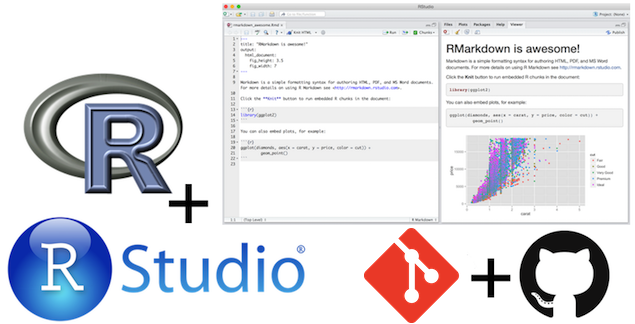
\includegraphics{img/toolkit.png}
\caption{R as a toolkit}
\end{figure}

\begin{itemize}
\tightlist
\item
  Scriptability \(\rightarrow\) R
\item
  Literate programming (code, narrative, output in one place) \(\rightarrow\) R Markdown
\item
  Version control \(\rightarrow\) Git / GitHub
\end{itemize}

\hypertarget{why-r-and-rstudio}{%
\subsection{Why R and RStudio?}\label{why-r-and-rstudio}}

\begin{flushright}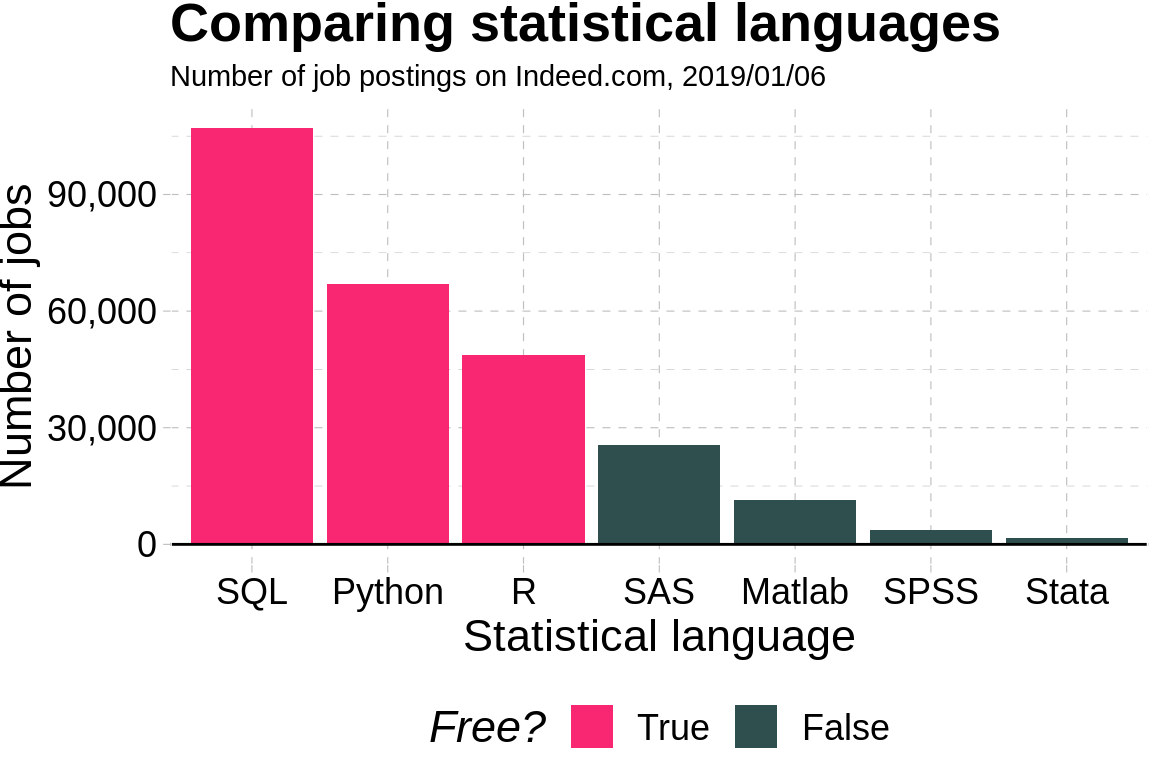
\includegraphics{vistransrep_files/figure-latex/indeeddotcom-1} \end{flushright}

\hypertarget{some-r-basics}{%
\subsection{Some R basics}\label{some-r-basics}}

\begin{itemize}
\tightlist
\item
  You will load packages at the \textbf{start of every new R session}.

  \begin{itemize}
  \tightlist
  \item
    ``Base'' R comes with tons of useful built-in functions. It also provides all the tools necessary for you to write your own functions.
  \item
    However, many of R's best data science functions and tools come from external packages written by other users.
  \end{itemize}
\item
  R easily and infinitely parallelizes. For free.

  \begin{itemize}
  \tightlist
  \item
    Compare the cost of a \href{https://www.stata.com/statamp/}{Stata/MP} license, nevermind the fact that you effectively pay per core\ldots{}
  \end{itemize}
\end{itemize}

\hypertarget{r-code-examples}{%
\section{R code examples}\label{r-code-examples}}

\hypertarget{linear-regression}{%
\subsection{Linear regression}\label{linear-regression}}

\begin{Shaded}
\begin{Highlighting}[]
\NormalTok{fit <-}\StringTok{ }\KeywordTok{lm}\NormalTok{(dist }\OperatorTok{~}\StringTok{ }\DecValTok{1} \OperatorTok{+}\StringTok{ }\NormalTok{speed, }\DataTypeTok{data =}\NormalTok{ cars)}
\KeywordTok{summary}\NormalTok{(fit)}
\end{Highlighting}
\end{Shaded}

\begin{verbatim}
## 
## Call:
## lm(formula = dist ~ 1 + speed, data = cars)
## 
## Residuals:
##     Min      1Q  Median      3Q     Max 
## -29.069  -9.525  -2.272   9.215  43.201 
## 
## Coefficients:
##             Estimate Std. Error t value Pr(>|t|)    
## (Intercept) -17.5791     6.7584  -2.601   0.0123 *  
## speed         3.9324     0.4155   9.464 1.49e-12 ***
## ---
## Signif. codes:  0 '***' 0.001 '**' 0.01 '*' 0.05 '.' 0.1 ' ' 1
## 
## Residual standard error: 15.38 on 48 degrees of freedom
## Multiple R-squared:  0.6511, Adjusted R-squared:  0.6438 
## F-statistic: 89.57 on 1 and 48 DF,  p-value: 1.49e-12
\end{verbatim}

\hypertarget{base-r-plot}{%
\subsection{Base R plot}\label{base-r-plot}}

\begin{Shaded}
\begin{Highlighting}[]
\KeywordTok{plot}\NormalTok{(cars, }\DataTypeTok{pch =} \DecValTok{19}\NormalTok{, }\DataTypeTok{col =} \StringTok{"darkgray"}\NormalTok{)}
\KeywordTok{abline}\NormalTok{(fit, }\DataTypeTok{lwd =} \DecValTok{2}\NormalTok{)}
\end{Highlighting}
\end{Shaded}

\begin{flushright}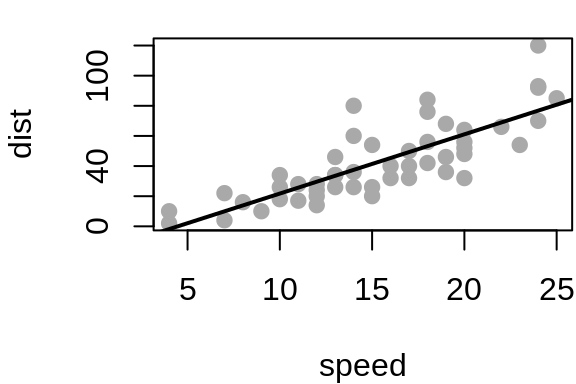
\includegraphics{vistransrep_files/figure-latex/cars_basefig-1} \end{flushright}

\hypertarget{ggplot2}{%
\subsection{ggplot2}\label{ggplot2}}

\begin{Shaded}
\begin{Highlighting}[]
\KeywordTok{library}\NormalTok{(ggplot2)}
\KeywordTok{library}\NormalTok{(gapminder) ## For the gapminder data}

\KeywordTok{ggplot}\NormalTok{(}
  \DataTypeTok{data =}\NormalTok{ gapminder,}
  \DataTypeTok{mapping =} \KeywordTok{aes}\NormalTok{(}\DataTypeTok{x =}\NormalTok{ gdpPercap, }\DataTypeTok{y =}\NormalTok{ lifeExp)}
\NormalTok{) }\OperatorTok{+}
\StringTok{  }\KeywordTok{geom_point}\NormalTok{()}
\end{Highlighting}
\end{Shaded}

\begin{flushright}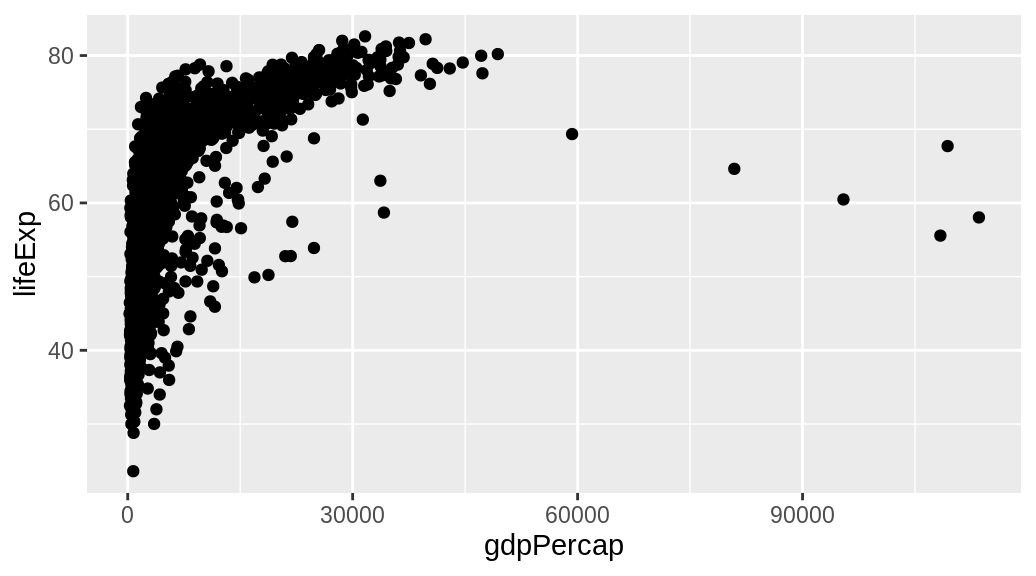
\includegraphics{vistransrep_files/figure-latex/gapm_plot-1} \end{flushright}

\hypertarget{gganimate}{%
\subsection{gganimate}\label{gganimate}}

\hypertarget{r-vs.rstudio}{%
\section{R vs.~RStudio}\label{r-vs.rstudio}}

\begin{itemize}
\tightlist
\item
  R is a statistical \textbf{programming language}
\item
  RStudio is a convenient interface for R (an \textbf{integrated development environment}, IDE)
\item
  At its simplest:

  \begin{itemize}
  \tightlist
  \item
    R is like a car's engine
  \item
    RStudio is like a car's dashboard
  \end{itemize}
\end{itemize}

\begin{figure}
\centering
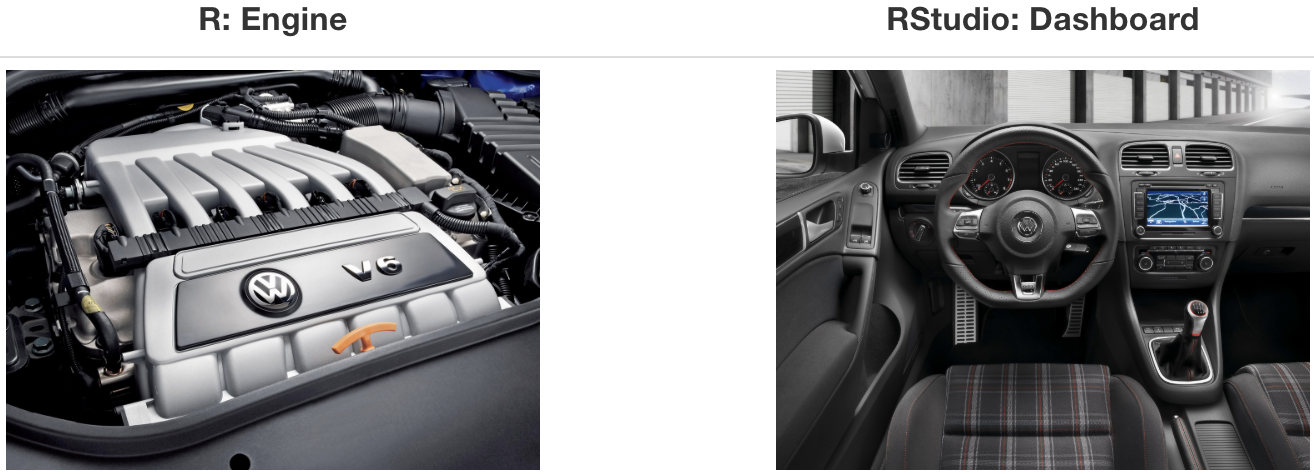
\includegraphics{img/engine-dashboard.png}
\caption{Engine vs.~dashboard}
\end{figure}

\hypertarget{r-vs.r-packages}{%
\section{R vs.~R packages}\label{r-vs.r-packages}}

\begin{itemize}
\item
  R packages \textbf{extend} the functionality of R by providing additional functions, data, and documentation.
\item
  They are written by a world-wide community of R users and can be downloaded for no cost
\end{itemize}

\begin{figure}
\centering
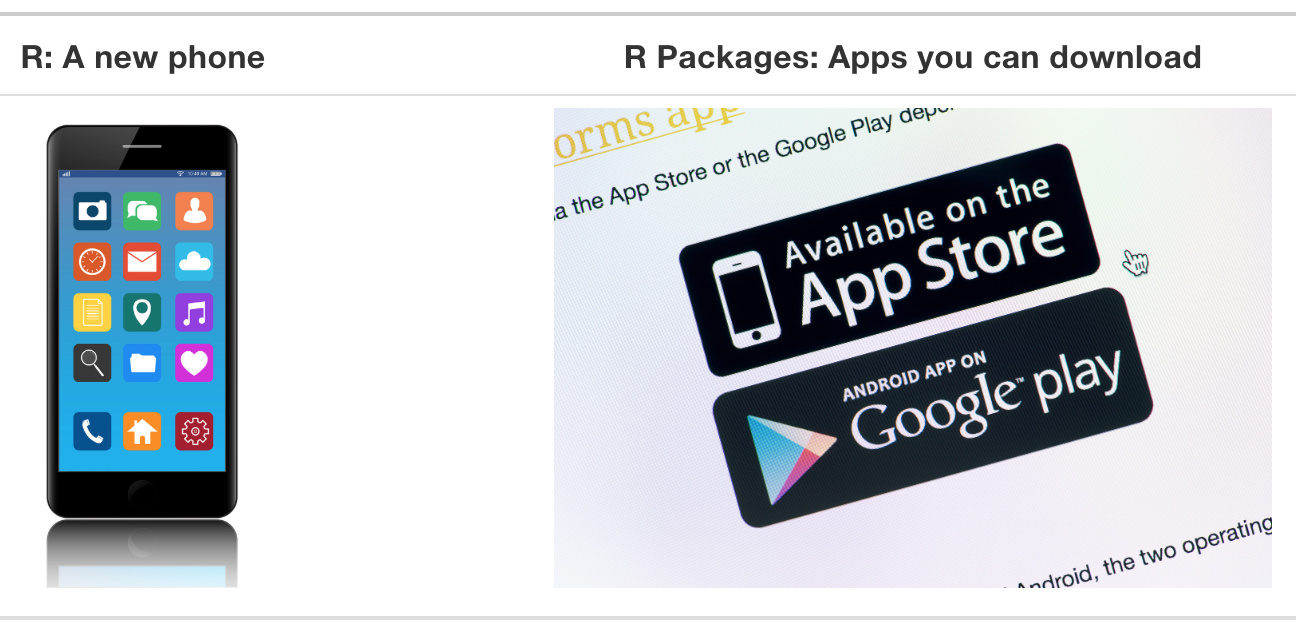
\includegraphics{img/r_vs_r_packages.png}
\caption{R versus R packages}
\end{figure}

\hypertarget{r-packages}{%
\section{R packages}\label{r-packages}}

\begin{itemize}
\item
  \textbf{CRAN}: A group of people who check that packages fulfill certain standards
\item
  \textbf{Mirror}: A location on the web where to download R packages from. Because many thousand people download them daily, the load is distributed on different machines. Pick one which is geographically close to you
\item
  \textbf{R base/recommended packages}: The base installation of R ships with a bunch of default packages. In addition, there are some more packages listed as ``recommended''.
\end{itemize}

``base'' packages are managed by the R core team and will only be updated for every R release.

Packages listed as ``recommended'' inherit the attributes of being widely used and having a long history in the R community.

\begin{verbatim}
##     Package Priority
## 1      base     base
## 2  compiler     base
## 3  datasets     base
## 4  graphics     base
## 5 grDevices     base
## 6      grid     base
## 7   methods     base
## 8  parallel     base
\end{verbatim}

\begin{verbatim}
##       Package    Priority
## 1        boot recommended
## 2       class recommended
## 3     cluster recommended
## 4   codetools recommended
## 5     foreign recommended
## 6  KernSmooth recommended
## 7     lattice recommended
## 8        MASS recommended
## 9      Matrix recommended
## 10       mgcv recommended
##  [ reached 'max' / getOption("max.print") -- omitted 2 rows ]
\end{verbatim}

\hypertarget{rprofile}{%
\section{.Rprofile}\label{rprofile}}

\begin{itemize}
\item
  File in your home directory \texttt{\textasciitilde{}/.Rprofile}
\item
  Will be executed before every R session starts
\item
  Useful to set global options and for loading of often used packages
\end{itemize}

\hypertarget{renviron}{%
\section{.Renviron}\label{renviron}}

\begin{itemize}
\item
  File in your home directory \texttt{\textasciitilde{}/.Renviron}
\item
  Used to set environment variables
\item
  Used to store ``Access tokens'' (Github, CI provider, C++ flags)
\end{itemize}

\hypertarget{rstudio}{%
\chapter{RStudio}\label{rstudio}}

\hypertarget{ide-structure}{%
\section{IDE structure}\label{ide-structure}}

\(\rightarrow\) Exists to \textbf{boost} your productivity

\(\rightarrow\) Change the defaults to your liking so you \emph{actually} can be \textbf{productive}

\(\rightarrow\) Keybindings = productivity

Since RStudio v1.3 a \href{https://docs.rstudio.com/ide/desktop-pro/latest/settings.html\#preferences}{portable JSON settings file} exists.

If you want to have sane settings without much hassle, you can execute the following R code: \texttt{source("https://bit.ly/rstudio-pat")}

This code will change/overwrite your existing RStudio settings and

\begin{itemize}
\item
  set custom keybindings
\item
  move the console panel to the top-right (by default bottom-left)
\item
  Enable/Disable some core settings to have a better overall experience
\end{itemize}

\begin{center}\rule{0.5\linewidth}{\linethickness}\end{center}

R scripts (source code) are written in the \emph{Source} pane (Editor).

\begin{figure}
\centering
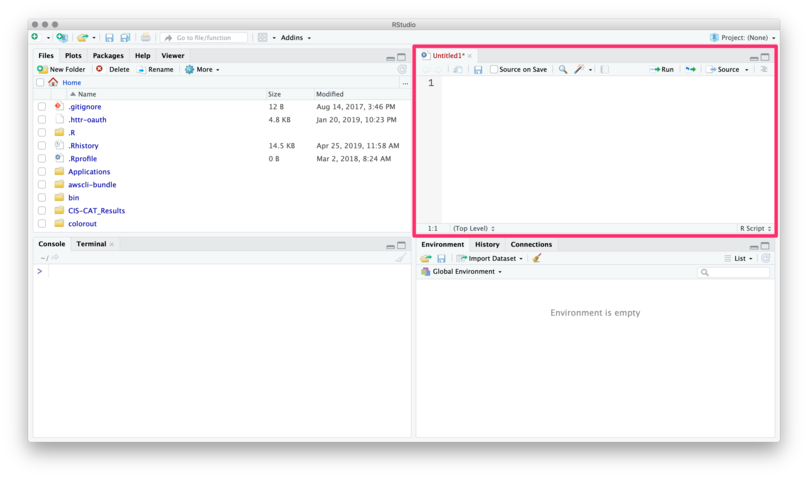
\includegraphics{img/rstudio_source_rec.png}
\caption{Source pane}
\end{figure}

(Source of all following RStudio screenshots: \url{https://github.com/edrubin/EC525S19})

\begin{center}\rule{0.5\linewidth}{\linethickness}\end{center}

You can use the menubar or ⇧+⌘+N / ⇧+CTRL+N to create new R scripts.

\begin{figure}
\centering
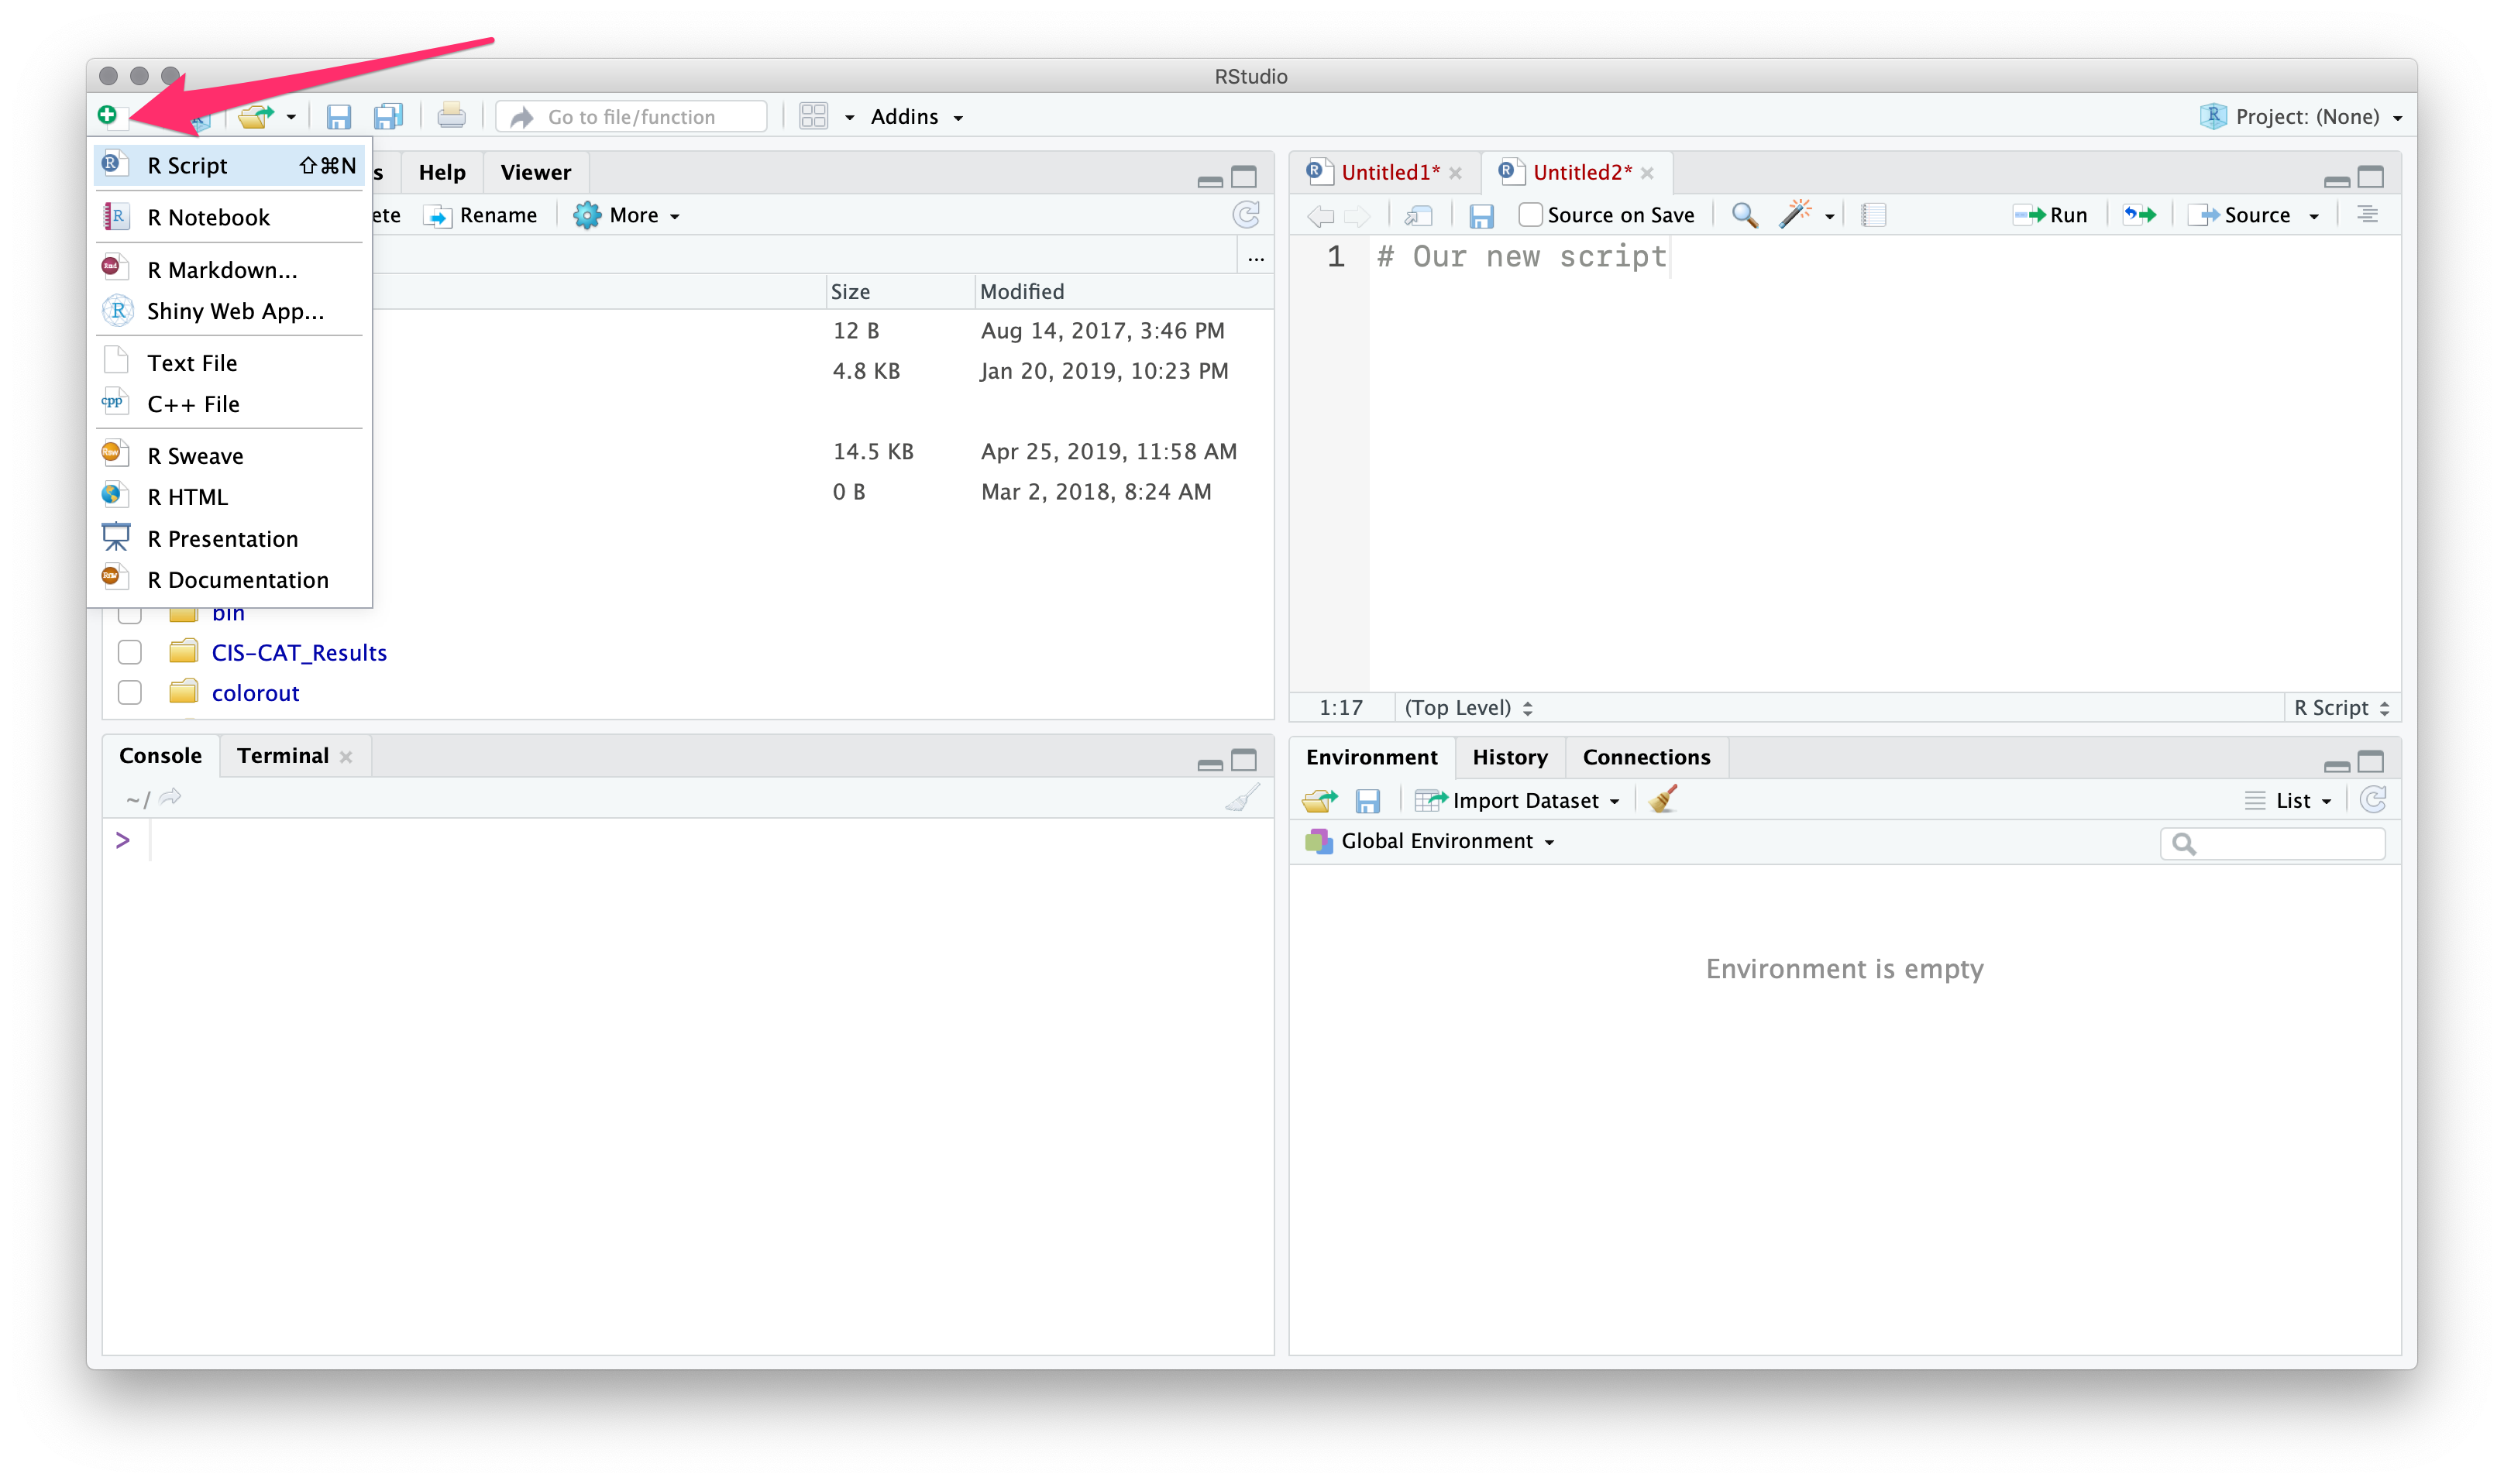
\includegraphics{img/rstudio_source_arrow.png}
\caption{New script}
\end{figure}

\begin{center}\rule{0.5\linewidth}{\linethickness}\end{center}

To execute commands from your R script, use ⌘+Enter / CTRL+Enter.

\begin{figure}
\centering
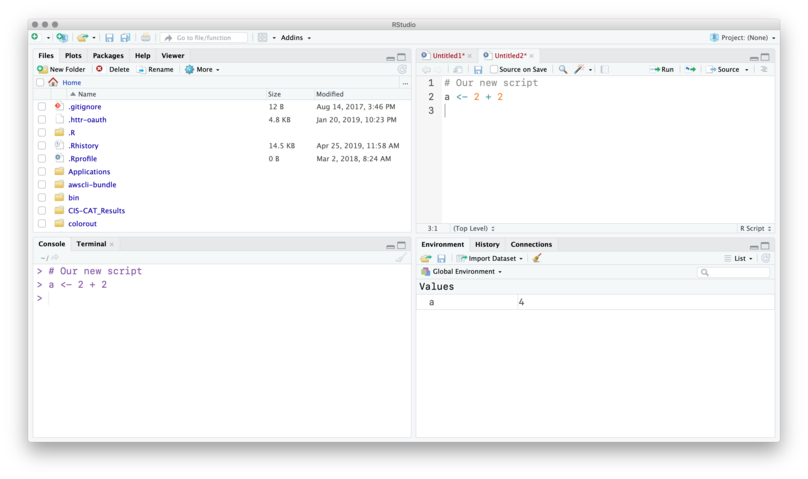
\includegraphics{img/rstudio_source_ex.png}
\caption{Execute commands}
\end{figure}

RStudio will execute the command in the console.

\begin{figure}
\centering
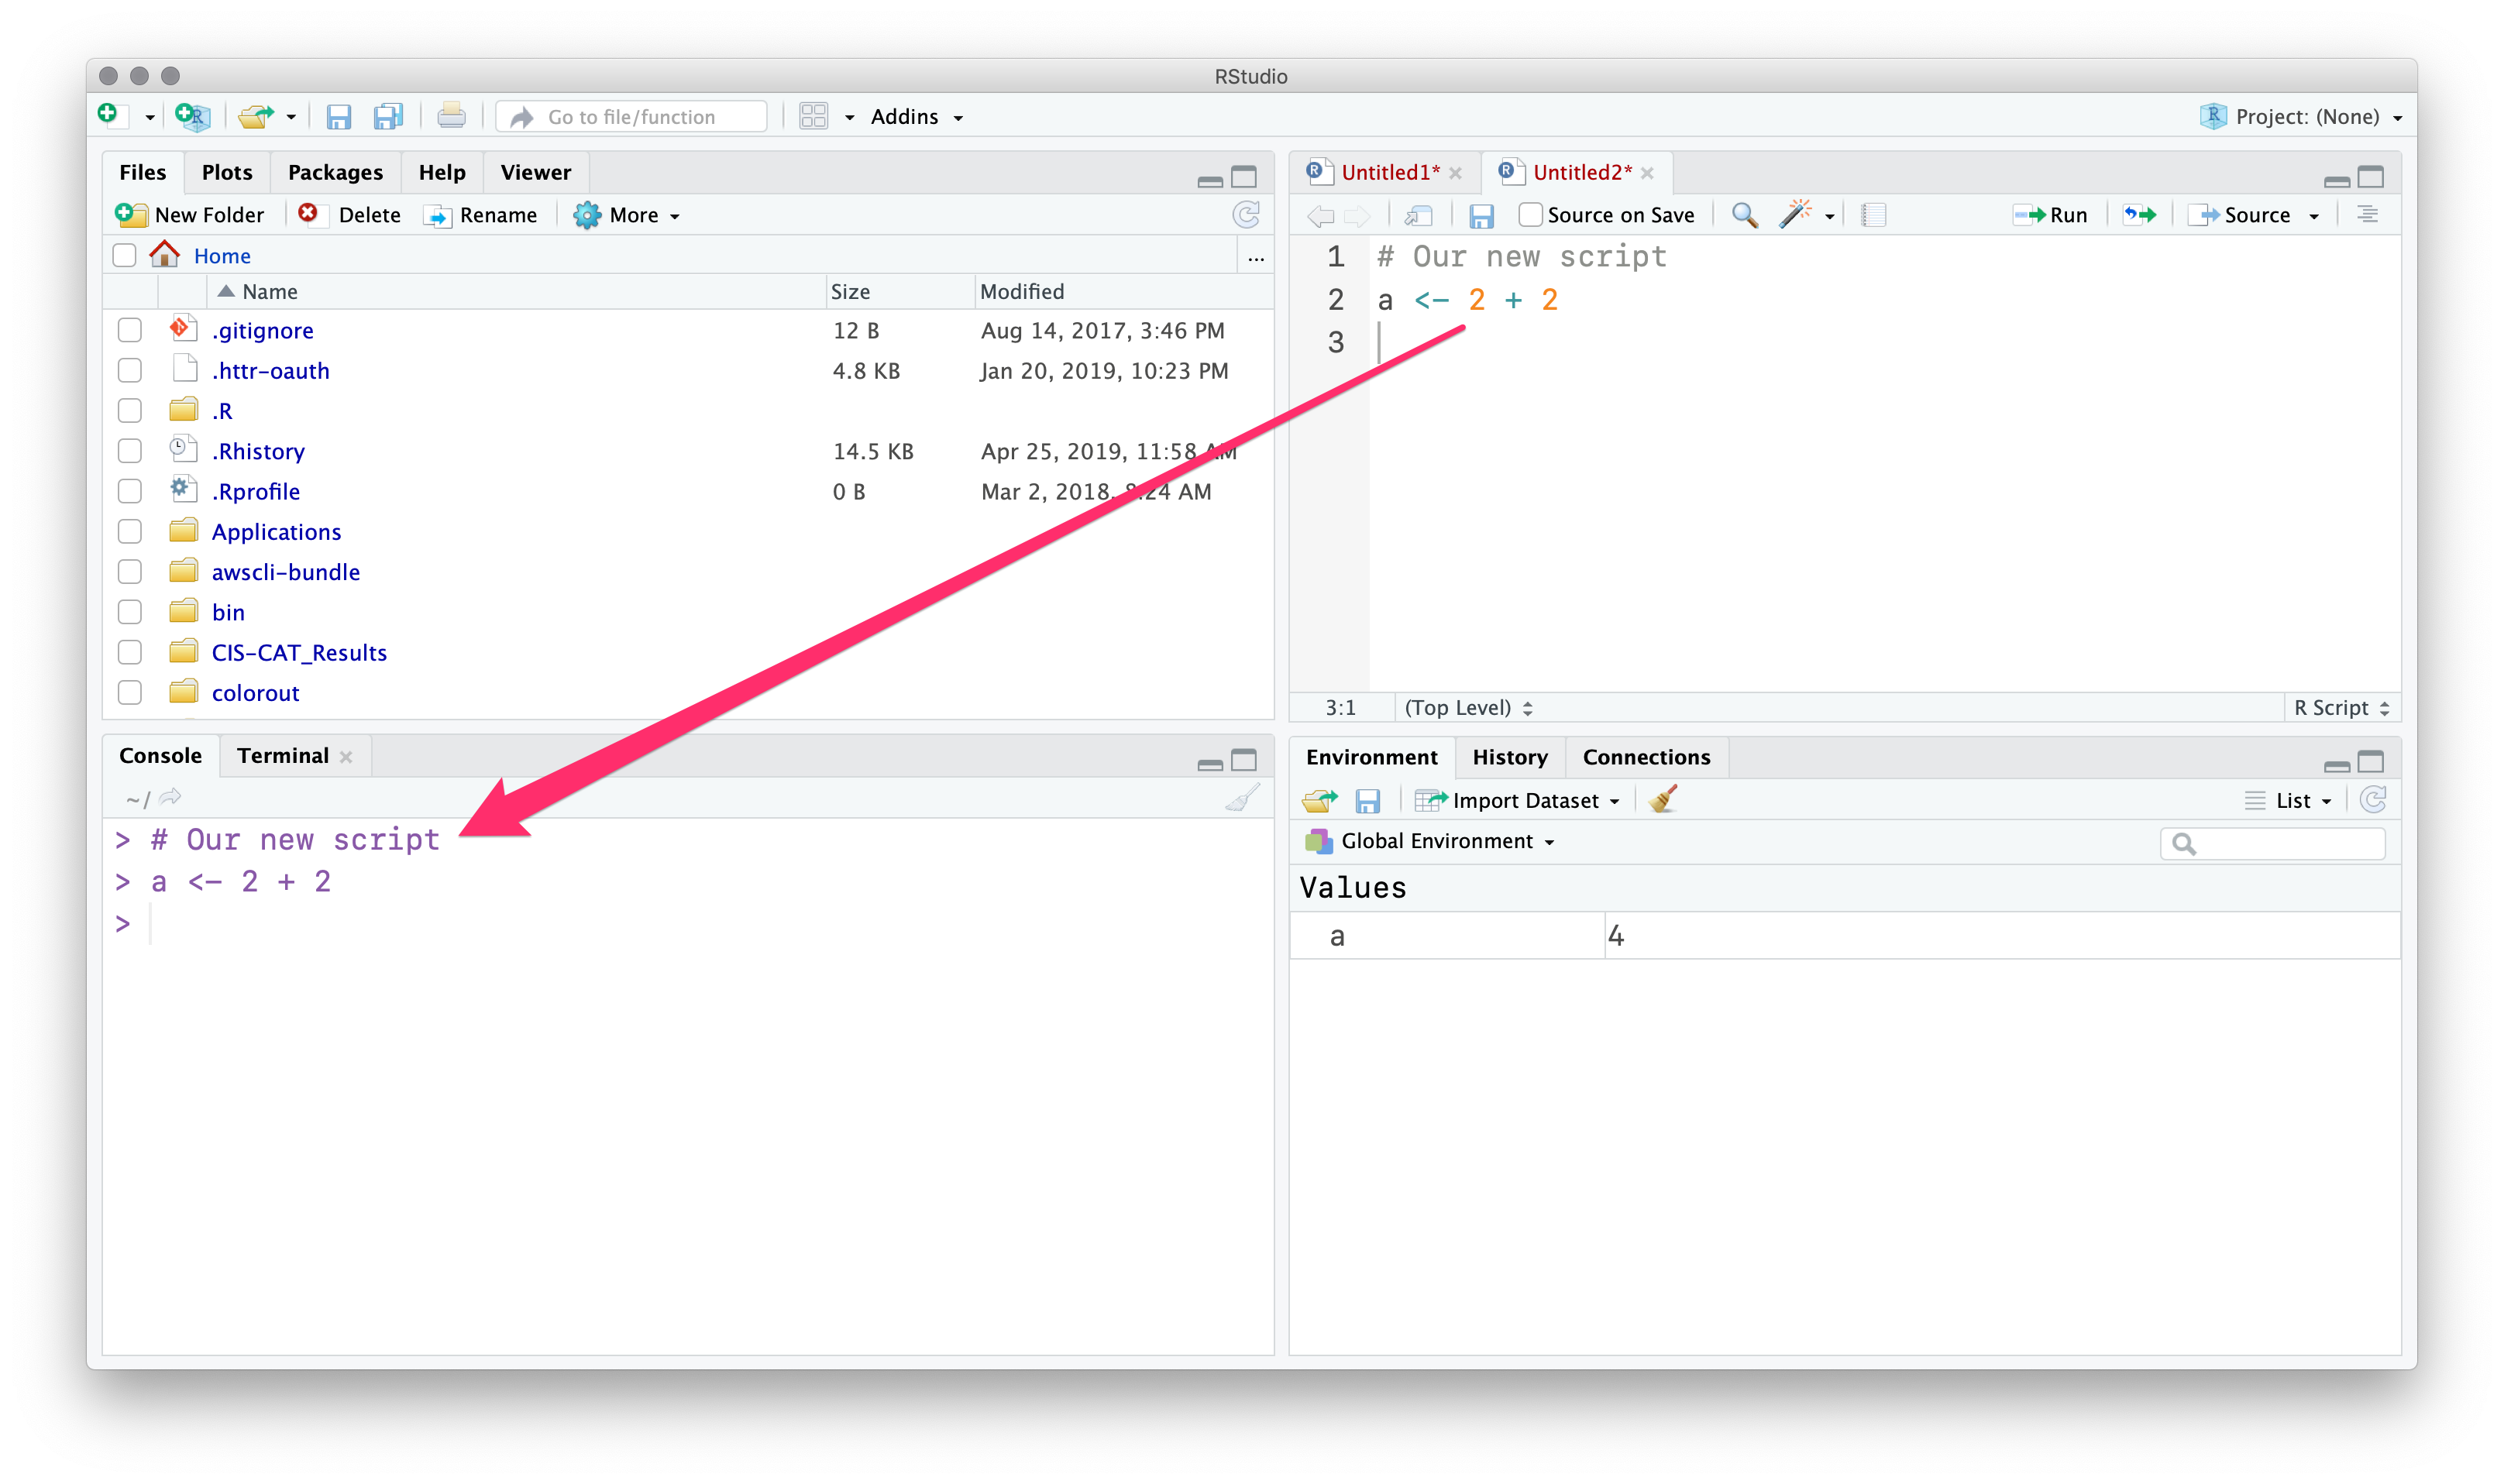
\includegraphics{img/rstudio_source_ex2.png}
\caption{Console output}
\end{figure}

You can see the new object in the \emph{Environment} pane.

\begin{figure}
\centering
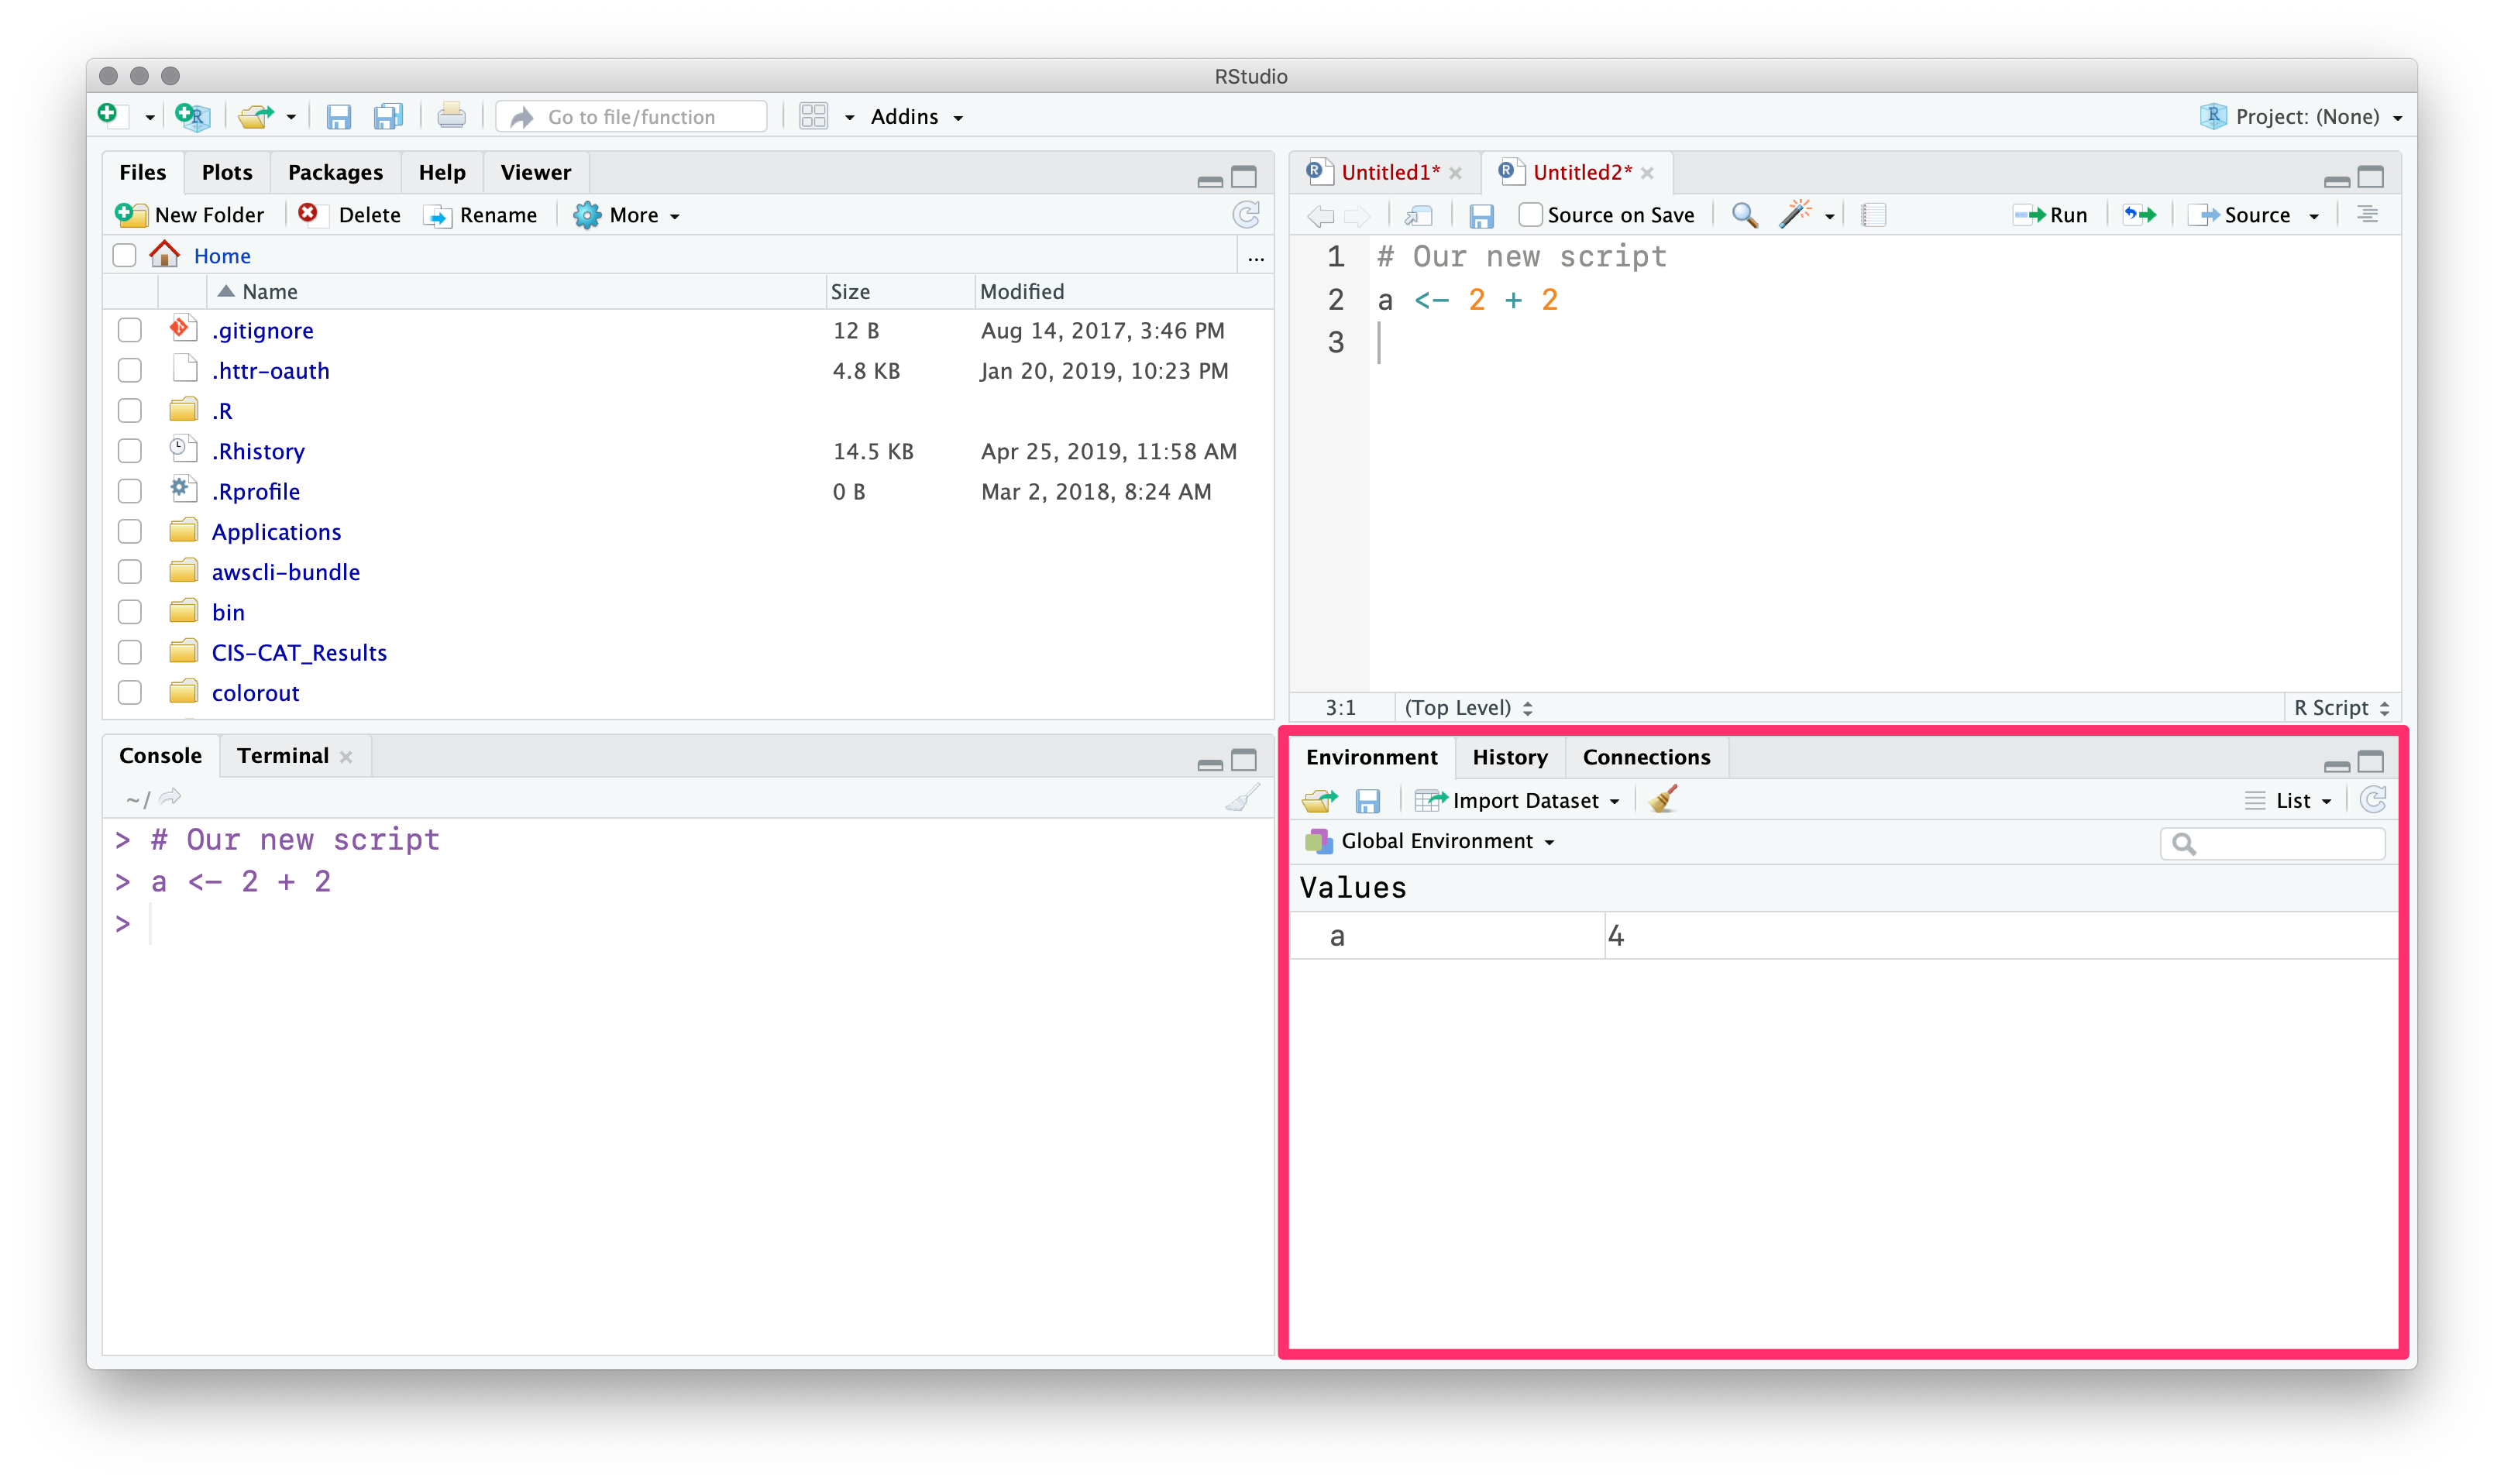
\includegraphics{img/rstudio_source_ex3.png}
\caption{Environment pane}
\end{figure}

\begin{center}\rule{0.5\linewidth}{\linethickness}\end{center}

The \emph{History} tab records your old commands.

\begin{figure}
\centering
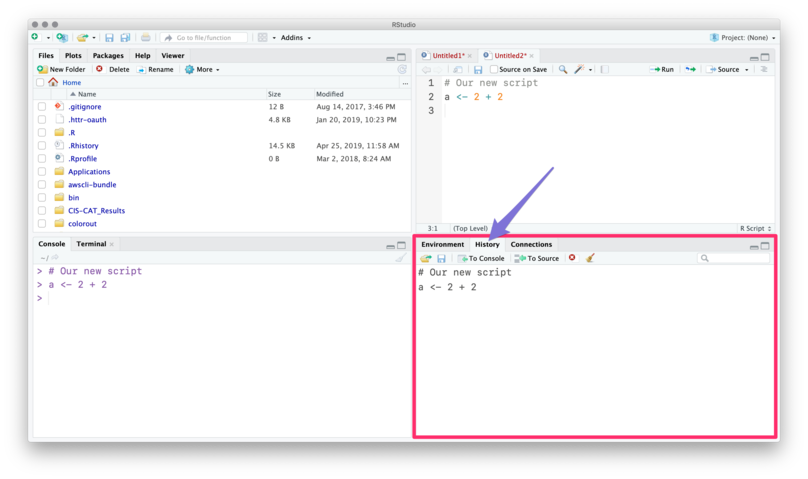
\includegraphics{img/rstudio_history.png}
\caption{History pane}
\end{figure}

\begin{center}\rule{0.5\linewidth}{\linethickness}\end{center}

The \emph{Files} pane is the file explorer.

\begin{figure}
\centering
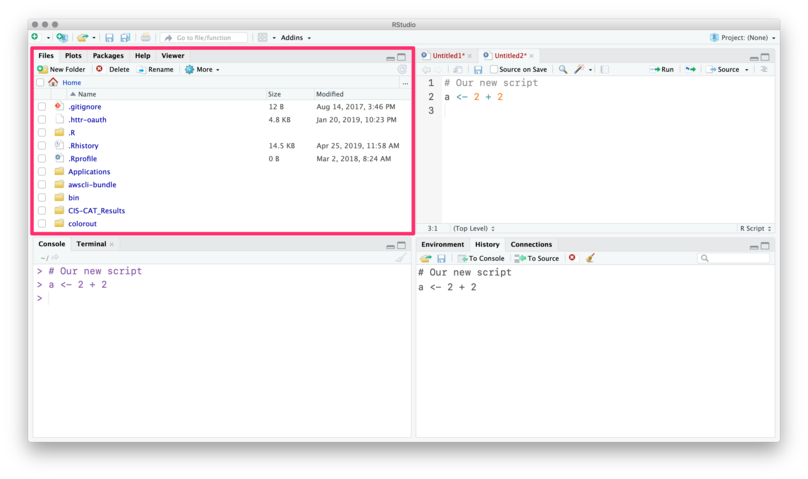
\includegraphics{img/rstudio_files.png}
\caption{Files pane}
\end{figure}

\begin{center}\rule{0.5\linewidth}{\linethickness}\end{center}

The \emph{Plots} pane/tab shows\ldots{} plots.

\begin{figure}
\centering
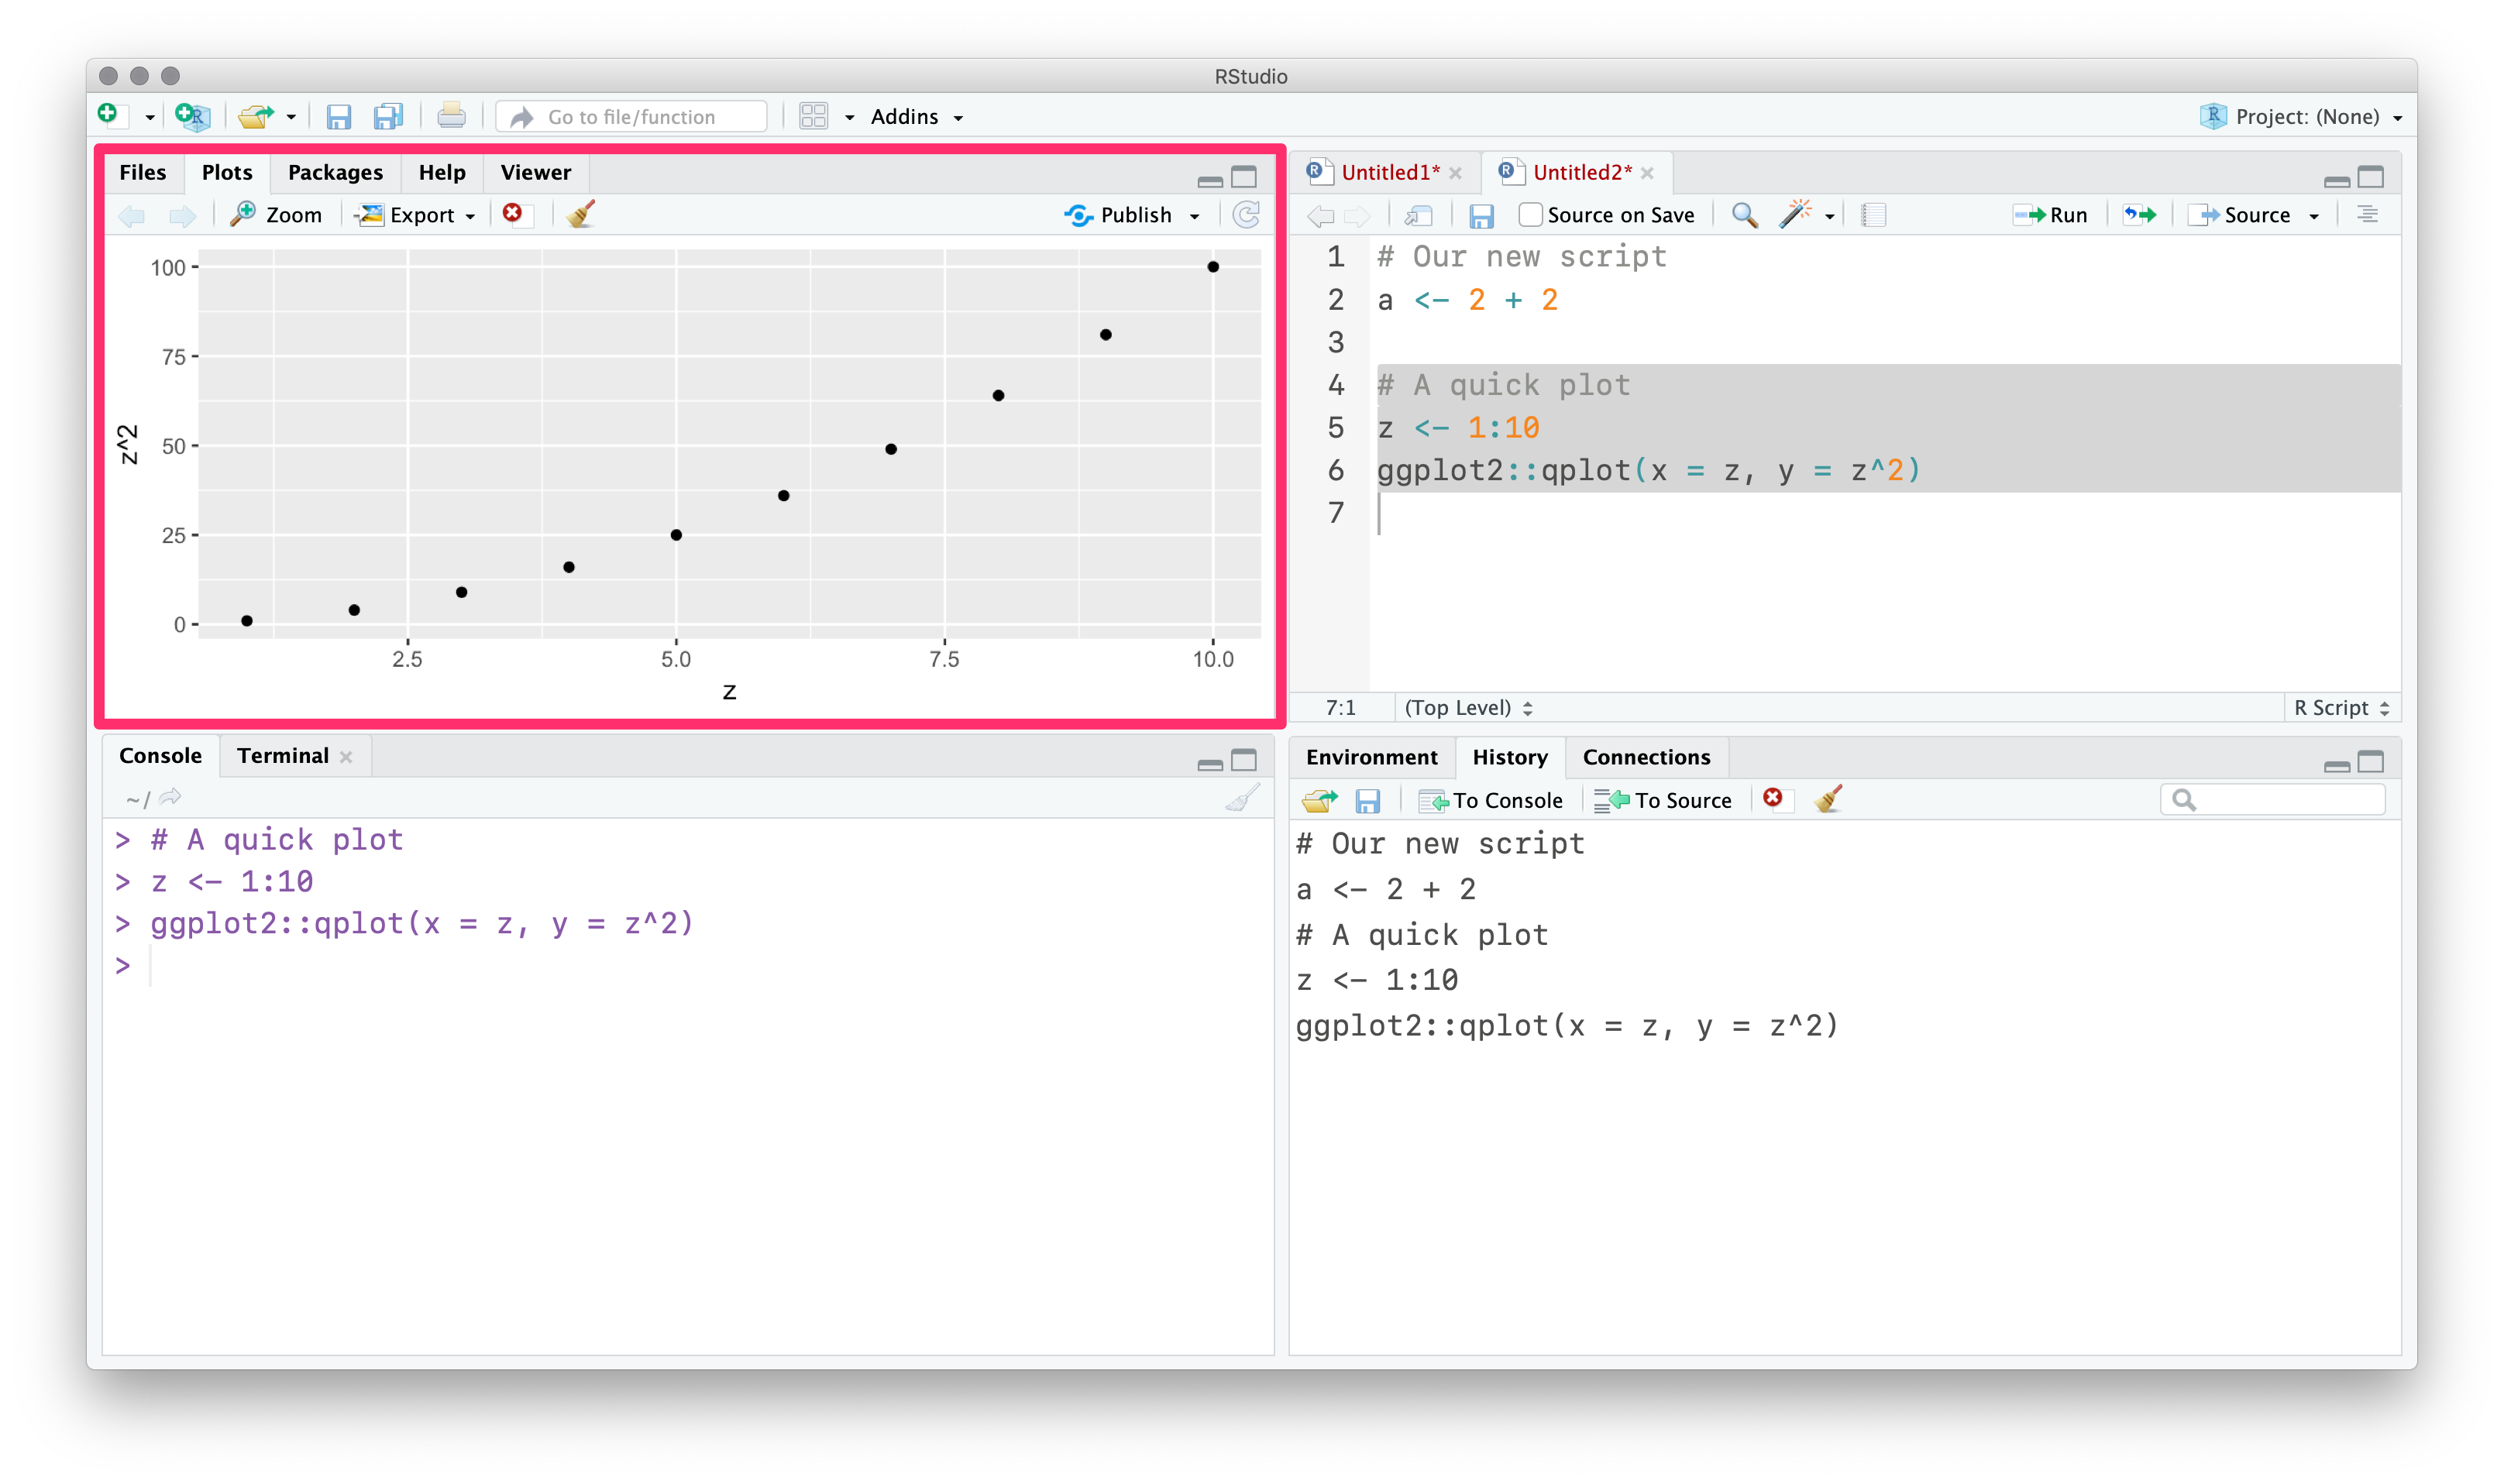
\includegraphics{img/rstudio_plots.png}
\caption{Plots pane}
\end{figure}

\begin{center}\rule{0.5\linewidth}{\linethickness}\end{center}

\emph{Packages} shows installed packages

\begin{figure}
\centering
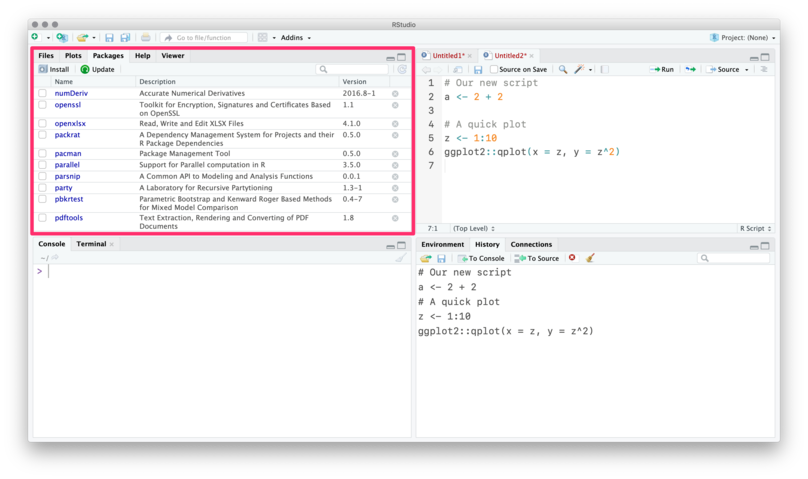
\includegraphics{img/rstudio_packages.png}
\caption{Packages pane}
\end{figure}

\begin{center}\rule{0.5\linewidth}{\linethickness}\end{center}

\emph{Packages} shows installed packages and whether they are \emph{loaded}.

\begin{figure}
\centering
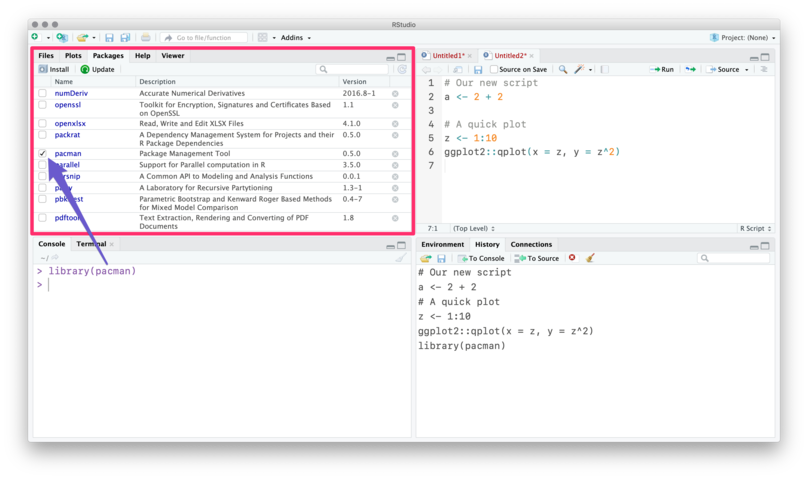
\includegraphics{img/rstudio_packages2.png}
\caption{Loaded and installed packages}
\end{figure}

\begin{center}\rule{0.5\linewidth}{\linethickness}\end{center}

The \emph{Help} tab shows help documentation (also accessible via \texttt{?}).

\begin{figure}
\centering
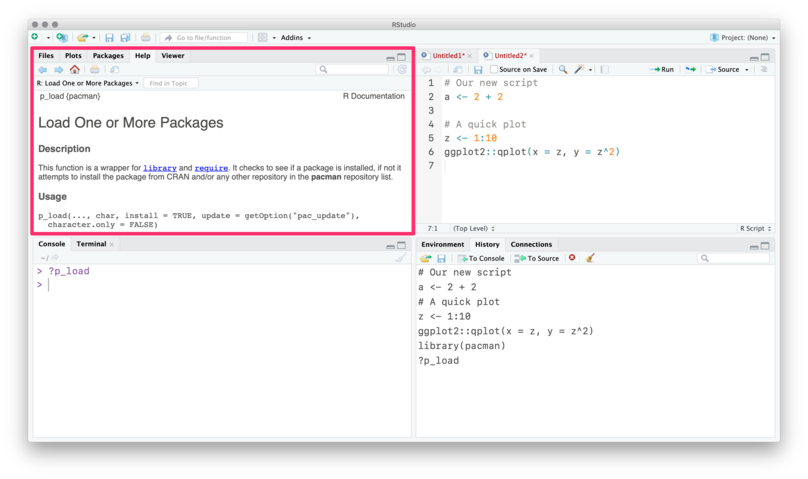
\includegraphics{img/rstudio_help.png}
\caption{Help pane}
\end{figure}

\begin{center}\rule{0.5\linewidth}{\linethickness}\end{center}

Finally, you can customize the actual layout

\begin{figure}
\centering
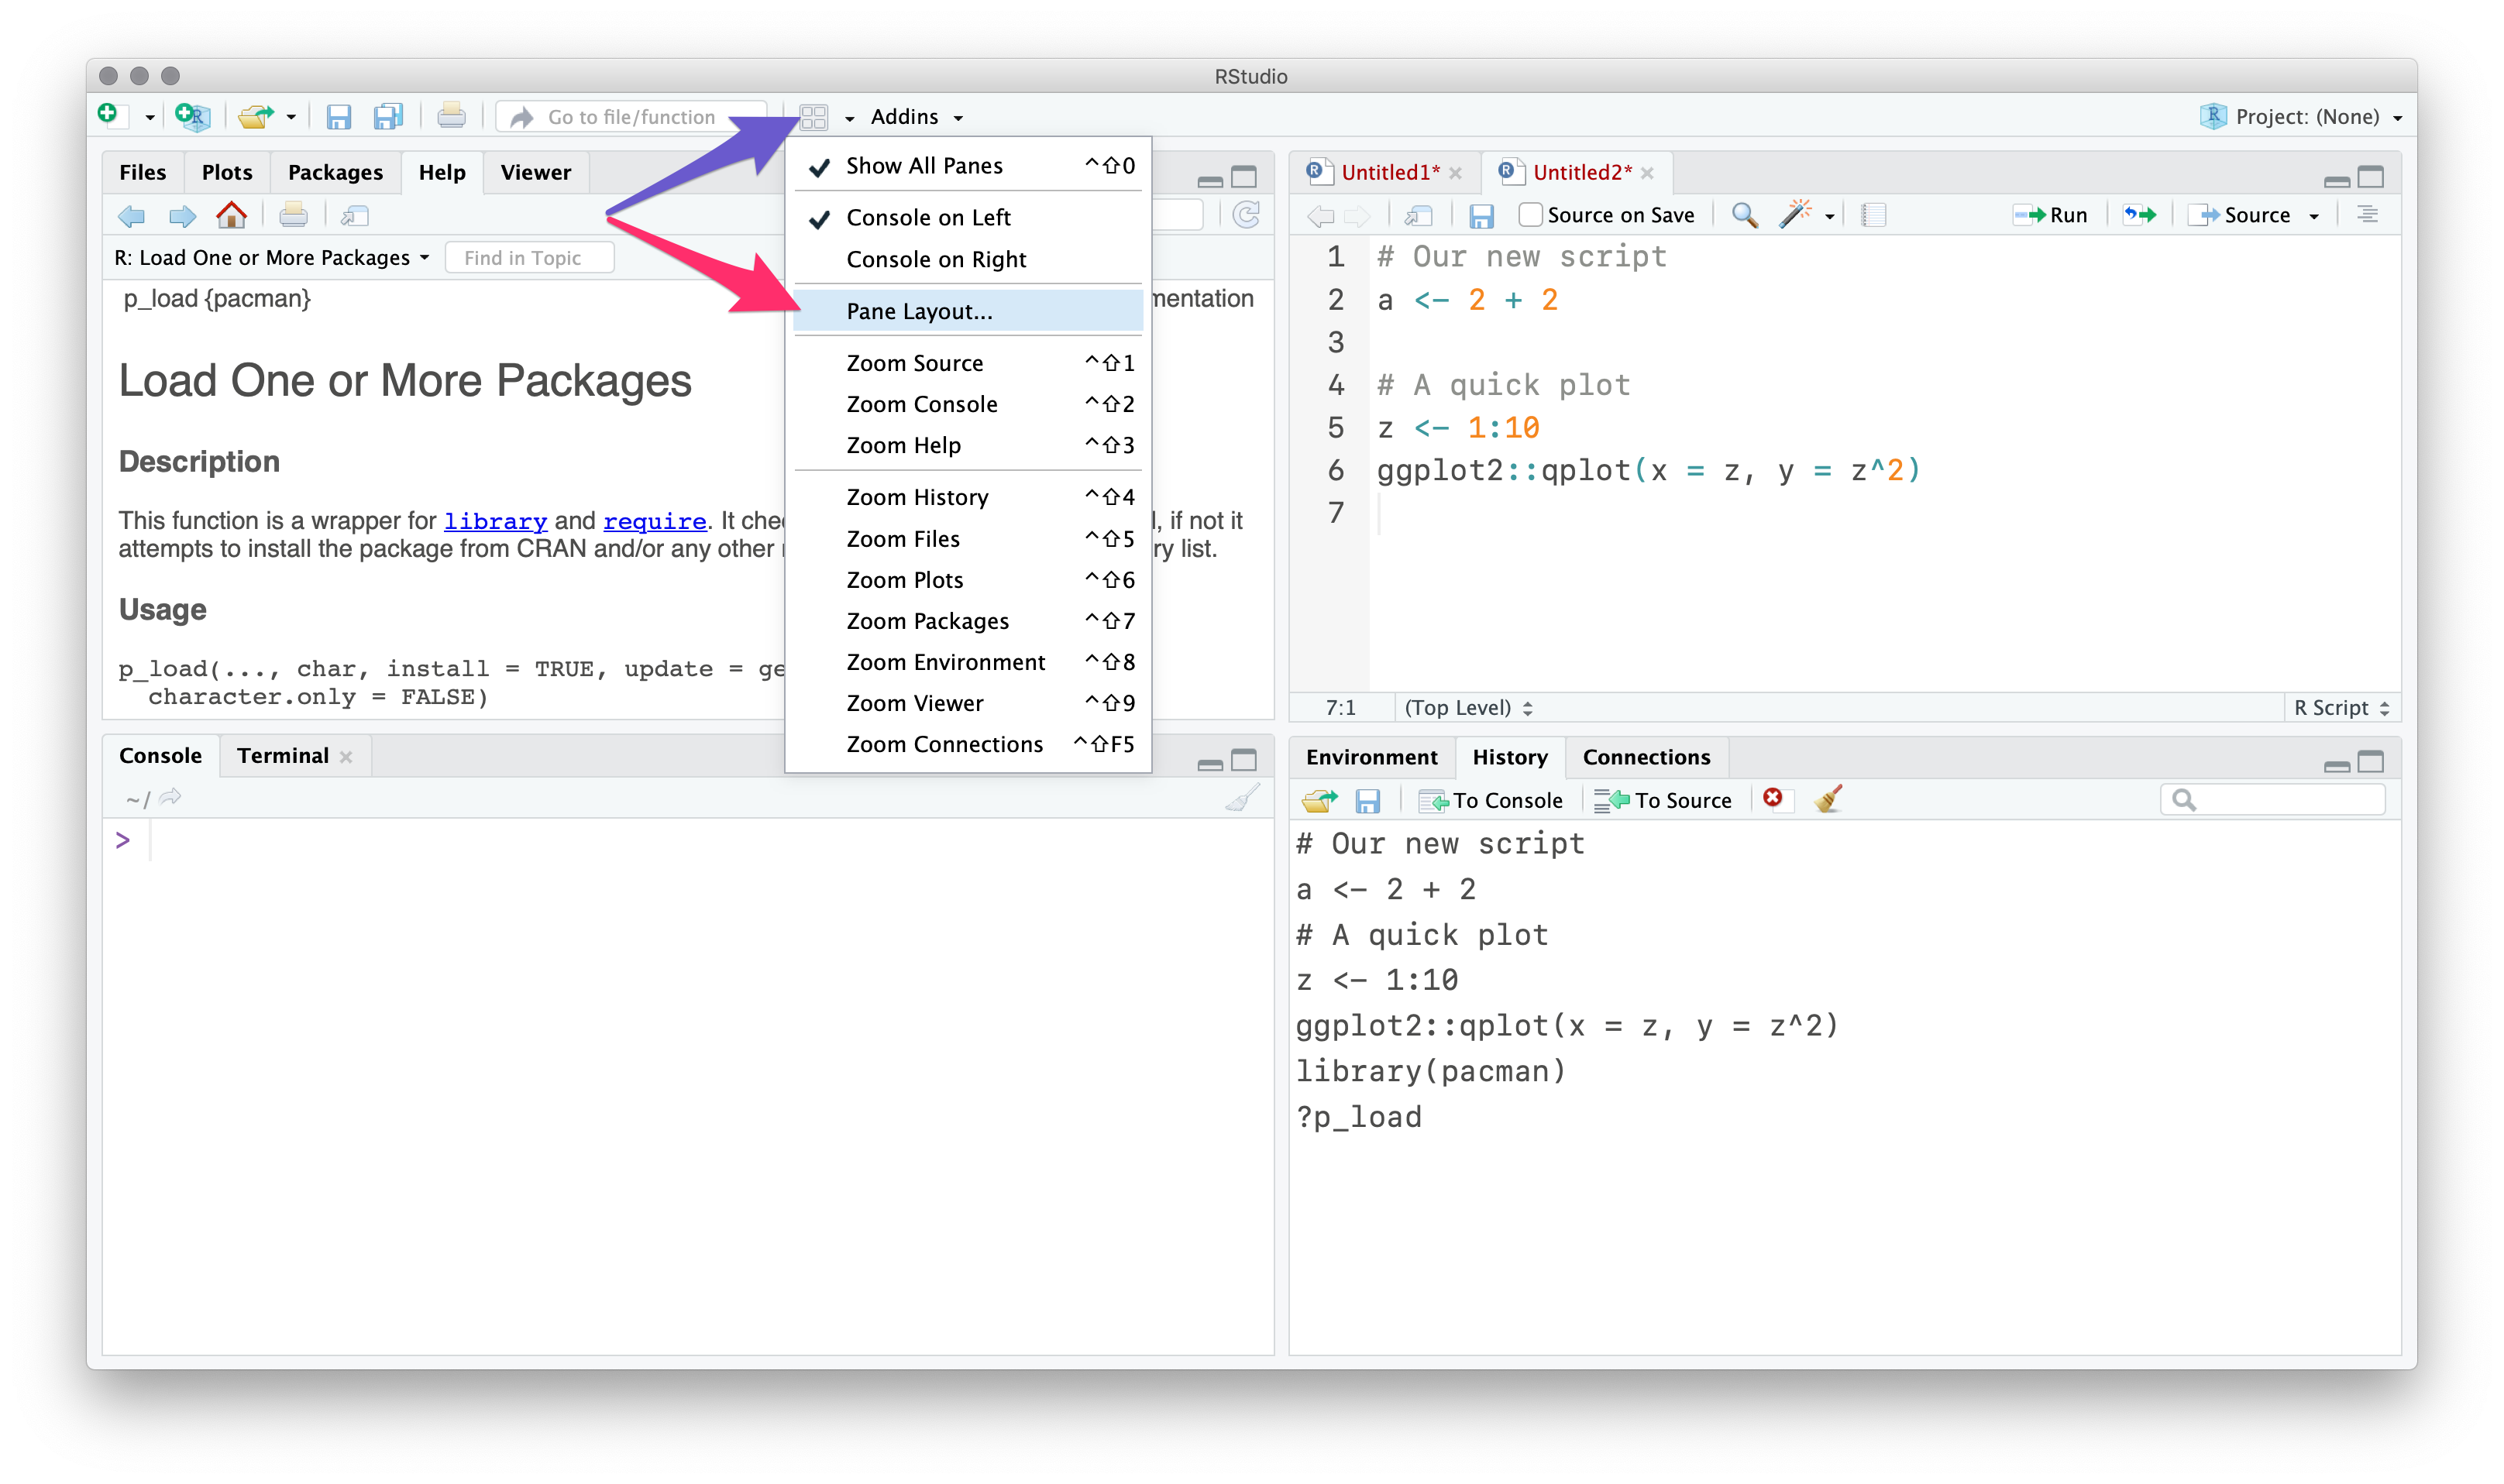
\includegraphics{img/rstudio_layout.png}
\caption{Customize layout}
\end{figure}

\hypertarget{rstudio-addins}{%
\section{RStudio Addins}\label{rstudio-addins}}

RStudio can be further enhanced by so called ``addins''.
These are clickable snippets that execute certain actions in RStudio.

They aim to make repetitive tasks easier and to save you time.
There is an addin called \href{https://github.com/daattali/addinslist}{addinslist} which lists all available addins.
It can be installed as a normal package from CRAN:

\texttt{install.packages("addinslist")}

To have an addin available in RStudio after installation, RStudio needs to be restarted.

\hypertarget{rstudio-projects}{%
\section{RStudio projects}\label{rstudio-projects}}

Without a project, you will need to define \textbf{long} file paths which \textbf{only exist on your machine}.

\begin{Shaded}
\begin{Highlighting}[]
\NormalTok{sample_df <-}\StringTok{ }\KeywordTok{read.csv}\NormalTok{(}\StringTok{"/Users/<yourname>/somewhere/on/this/machine/sample.csv"}\NormalTok{)}
\end{Highlighting}
\end{Shaded}

With a project, R automatically references the project's folder as the current working directory.

From there on, you can use \emph{relative paths} to point to files.

\begin{Shaded}
\begin{Highlighting}[]
\NormalTok{sample_df <-}\StringTok{ }\KeywordTok{read.csv}\NormalTok{(}\StringTok{"sample.csv"}\NormalTok{)}
\end{Highlighting}
\end{Shaded}

\textbf{Double-plus bonus}: The \href{https://github.com/r-lib/here}{\emph{here}} package extends \emph{RStudio project} philosophy even more and helps in cases when not using RStudio (e.g.~on the command line).

\hypertarget{alternatives-to-rstudio}{%
\section{Alternatives to RStudio}\label{alternatives-to-rstudio}}

\begin{itemize}
\item
  Using R directly in the terminal via \href{https://github.com/randy3k/radian}{radian} (optimized R console interpreter)
\item
  R is supported in other ``general purpose IDE's'' (VScode, Sublime Text, Atom, Vim, etc.)
\end{itemize}

\hypertarget{part-visualization}{%
\part{Visualization}\label{part-visualization}}

\hypertarget{vis-basics}{%
\chapter{\{ggplot2\} basics}\label{vis-basics}}

\begin{quote}
Embracing the grammar of graphics.
\end{quote}

This chapter discusses plotting with the \href{https://ggplot2.tidyverse.org/}{ggplot2 package}.

\hypertarget{vis-adv}{%
\chapter{\{ggplot2\} advanced}\label{vis-adv}}

\hypertarget{part-tidying-and-transforming}{%
\part{Tidying and transforming}\label{part-tidying-and-transforming}}

\hypertarget{import}{%
\chapter{Import}\label{import}}

\begin{quote}
Ingesting data.
\end{quote}

This chapter discusses data import with RStudio, with the help of the \href{https://readr.tidyverse.org/}{readr}, \href{https://readxl.tidyverse.org/}{readxl}, and \href{https://github.com/leeper/rio}{rio} packages.

\hypertarget{transformation}{%
\chapter{Transformation}\label{transformation}}

\begin{quote}
Using a consistent grammar of data manipulation.
\end{quote}

This chapter discusses data transformation with the \href{https://dplyr.tidyverse.org/}{dplyr package}.

\hypertarget{tidying}{%
\chapter{Tidying}\label{tidying}}

\begin{quote}
Rows, columns, cells.
\end{quote}

This chapter discusses pivoting and data tidying with the help of the \href{https://tidyr.tidyverse.org/}{tidyr} package.

\hypertarget{part-reporting}{%
\part{Reporting}\label{part-reporting}}

\hypertarget{part-appendix}{%
\part{Appendix}\label{part-appendix}}

\hypertarget{best-practices}{%
\chapter{Best practices}\label{best-practices}}

R code is often organized in packages that can be installed from centralized repositories such as CRAN or GitHub.
If you are new to writing R packages, this course cannot give a complete introduction into packages.
It is still useful to embrace some very few concepts of R packages to gain access to a vast toolbox and also organize your code in a standardized way familiar to other users.
With the first steps in place, the road to your first R package may become less steep.

\begin{itemize}
\tightlist
\item
  Create a \texttt{DESCRIPTION} file to declare dependencies and allow easy reloading of the functions you define
\item
  Store your functions in \texttt{.R} files in the \texttt{R/} directory in your project

  \begin{itemize}
  \tightlist
  \item
    Scripts that you execute live in \texttt{script/} or a similar directory
  \end{itemize}
\item
  Use \href{https://github.com/klutometis/roxygen}{roxygen2} to document your functions close to the source
\item
  Write tests for your functions, e.g.~with \href{https://testthat.r-lib.org/}{testthat}
\end{itemize}

See \href{http://r-pkgs.had.co.nz/}{R packages} for a more comprehensive treatment.

\hypertarget{description}{%
\section{DESCRIPTION}\label{description}}

Create and open a new RStudio project.
Then, create a \texttt{DESCRIPTION} file with \texttt{usethis::use\_description()}:

\begin{Shaded}
\begin{Highlighting}[]
\CommentTok{# install.packages("usethis")}
\NormalTok{usethis}\OperatorTok{::}\KeywordTok{use_description}\NormalTok{()}
\end{Highlighting}
\end{Shaded}

Double-check success:

\begin{Shaded}
\begin{Highlighting}[]
\CommentTok{# install.packages("devtools")}
\NormalTok{devtools}\OperatorTok{::}\KeywordTok{load_all}\NormalTok{()}
\end{Highlighting}
\end{Shaded}

Declare that your project requires the tidyverse and the here package:

\begin{Shaded}
\begin{Highlighting}[]
\NormalTok{usethis}\OperatorTok{::}\KeywordTok{use_package}\NormalTok{(}\StringTok{"here"}\NormalTok{)}
\CommentTok{# Currently doesn't work, add manually}
\CommentTok{# https://github.com/r-lib/usethis/issues/760}
\CommentTok{# usethis::use_package("tidyverse")}
\end{Highlighting}
\end{Shaded}

\hypertarget{r-1}{%
\section{R}\label{r-1}}

With a \texttt{DESCRIPTION} file defined, create a new \texttt{.R} file and save it in the \texttt{R/} directory.
(Create this directory if it does not exist.)
Create a function in this file, save the file:

\begin{Shaded}
\begin{Highlighting}[]
\NormalTok{hi <-}\StringTok{ }\ControlFlowTok{function}\NormalTok{(}\DataTypeTok{text =} \StringTok{"Hello, world!"}\NormalTok{) \{}
  \KeywordTok{print}\NormalTok{(text)}
  \KeywordTok{invisible}\NormalTok{(text)}
\NormalTok{\}}
\end{Highlighting}
\end{Shaded}

Do not source the file.

Restart R (with Ctrl + Shift + F10 in RStudio).

Run \texttt{devtools::load\_all()} again, you can use the shortcut Ctrl + Shift + L or Cmd + Shift + L in RStudio.

Check that you can run \texttt{hi()} in the console:

\begin{Shaded}
\begin{Highlighting}[]
\KeywordTok{hi}\NormalTok{()}
\end{Highlighting}
\end{Shaded}

\begin{verbatim}
## [1] "Hello, world!"
\end{verbatim}

\begin{Shaded}
\begin{Highlighting}[]
\KeywordTok{hi}\NormalTok{(}\StringTok{"Wow!"}\NormalTok{)}
\end{Highlighting}
\end{Shaded}

\begin{verbatim}
## [1] "Wow!"
\end{verbatim}

Edit the function:

\begin{Shaded}
\begin{Highlighting}[]
\NormalTok{hi <-}\StringTok{ }\ControlFlowTok{function}\NormalTok{(}\DataTypeTok{text =} \StringTok{"Wow!"}\NormalTok{) \{}
  \KeywordTok{print}\NormalTok{(text)}
  \KeywordTok{invisible}\NormalTok{(text)}
\NormalTok{\}}
\end{Highlighting}
\end{Shaded}

Save the file, but do not source it.

Run \texttt{devtools::load\_all()} again, you can use the shortcut Ctrl + Shift + L or Cmd + Shift + L in RStudio.

Check that the new implementation of \texttt{hi()} is active:

\begin{Shaded}
\begin{Highlighting}[]
\KeywordTok{hi}\NormalTok{()}
\end{Highlighting}
\end{Shaded}

\begin{verbatim}
## [1] "Wow!"
\end{verbatim}

All functions that are required for your project are stored in this directory.
Do not store executable scripts, use a \texttt{script/} directory.

\hypertarget{roxygen2}{%
\section{roxygen2}\label{roxygen2}}

The following intuitive annotation syntax is a standard way to create documentation for your functions:

\begin{Shaded}
\begin{Highlighting}[]
\CommentTok{#' Print a welcome message}
\CommentTok{#' }
\CommentTok{#' This function prints "Wow!", or a custom text, on the console.}
\CommentTok{#'}
\CommentTok{#' @param text The text to print, "Wow!" by default.}
\CommentTok{#' }
\CommentTok{#' @return The `text` argument, invisibly.}
\CommentTok{#' }
\CommentTok{#' @examples}
\CommentTok{#' hi()}
\CommentTok{#' hi("Hello!")}
\NormalTok{hi <-}\StringTok{ }\ControlFlowTok{function}\NormalTok{(}\DataTypeTok{text =} \StringTok{"Wow!"}\NormalTok{) \{}
  \KeywordTok{print}\NormalTok{(text)}
  \KeywordTok{invisible}\NormalTok{(text)}
\NormalTok{\}}
\end{Highlighting}
\end{Shaded}

This annotation can be rendered to a nicely looking HTML page with the roxygen2 and pkgdown packages.
All you need to do is provide (and maintain) it.

\hypertarget{testthat}{%
\section{testthat}\label{testthat}}

Automated tests make sure that the functions you write today continue working tomorrow.
Create your first test with \texttt{usethis::use\_test()}:

\begin{Shaded}
\begin{Highlighting}[]
\CommentTok{# install.packages("testthat")}
\NormalTok{usethis}\OperatorTok{::}\KeywordTok{use_test}\NormalTok{(}\StringTok{"hi"}\NormalTok{)}
\end{Highlighting}
\end{Shaded}

The file \texttt{tests/testthat/test-hi.R} is created, with the following contents:

\begin{Shaded}
\begin{Highlighting}[]
\KeywordTok{test_that}\NormalTok{(}\StringTok{"multiplication works"}\NormalTok{, \{}
  \KeywordTok{expect_equal}\NormalTok{(}\DecValTok{2} \OperatorTok{*}\StringTok{ }\DecValTok{2}\NormalTok{, }\DecValTok{4}\NormalTok{)}
\NormalTok{\})}
\end{Highlighting}
\end{Shaded}

Replace this predefined text with a test that makes more sense for us:

\begin{Shaded}
\begin{Highlighting}[]
\KeywordTok{test_that}\NormalTok{(}\StringTok{"hi() works"}\NormalTok{, \{}
  \KeywordTok{expect_output}\NormalTok{(}\KeywordTok{hi}\NormalTok{(), }\StringTok{"Wow"}\NormalTok{)}
  \KeywordTok{expect_output}\NormalTok{(}\KeywordTok{hi}\NormalTok{(}\StringTok{"Hello"}\NormalTok{), }\StringTok{"Hello"}\NormalTok{)}
\NormalTok{\})}
\end{Highlighting}
\end{Shaded}

Run the new test with \texttt{devtools::test()}, you can use the shortcut Ctrl + Shift + T or Cmd + Shift + T in RStudio.

Check that the test actually detects failures by modifying the implementation of \texttt{hi()} and rerunning the test:

\begin{Shaded}
\begin{Highlighting}[]
\NormalTok{hi <-}\StringTok{ }\ControlFlowTok{function}\NormalTok{(}\DataTypeTok{text =} \StringTok{"Oops!"}\NormalTok{) \{}
  \KeywordTok{print}\NormalTok{(text)}
  \KeywordTok{invisible}\NormalTok{(text)}
\NormalTok{\}}
\end{Highlighting}
\end{Shaded}

Run the new test with \texttt{devtools::test()}, you can use the shortcut Ctrl + Shift + T or Cmd + Shift + T in RStudio.
One test should be failing now.

\hypertarget{section}{%
\chapter{}\label{section}}

\begin{itemize}
\item
  R for data science: \url{https://r4ds.had.co.nz/}
\item
  Row oriented workflows: \url{https://github.com/jennybc/row-oriented-workflows\#readme}
\item
  Advanced R: \url{http://adv-r.had.co.nz/}
\item
  Tidy evaluation: \url{https://tidyeval.tidyverse.org/}
\item
  R packages: \url{http://r-pkgs.had.co.nz/}
\item
  roxygen2: Vignettes in \url{https://cran.r-project.org/package=roxygen2}, especially:

  \begin{itemize}
  \item
    \href{https://cran.r-project.org/web/packages/roxygen2/vignettes/roxygen2.html}{Introduction to roxygen2}
  \item
    \href{https://cran.r-project.org/web/packages/roxygen2/vignettes/rd.html}{Generating Rd files} for an overview of available tags
  \item
    \href{https://cran.r-project.org/web/packages/roxygen2/vignettes/markdown.html}{Write R documentation in Markdown}
  \end{itemize}
\item
  How R searches and finds stuff: \url{http://blog.obeautifulcode.com/R/How-R-Searches-And-Finds-Stuff/}
\item
  What they forgot to teach you: \url{https://whattheyforgot.org/}
\item
  Parallel processing with a purrr-like interface: \url{https://davisvaughan.github.io/furrr/}
\item
  Tidyverse principles: \url{https://principles.tidyverse.org/}
\item
  Recursive lists to use in teaching and examples: \url{https://github.com/jennybc/repurrrsive}
\end{itemize}

\bibliography{book.bib}


\end{document}
